\documentclass[conference]{IEEEtran}
% IEEE conference version. Every number comes from generated macros (../macros.tex, ../macros_sensitivity.tex,
% ../macros_typeset.tex) or generated tables (../tables/*.tex), built by `python -m nycemis paper`, `sensitivity` and
% `report`. Do not type results here. Compiles with XeTeX (tectonic) and with pdfLaTeX.
\usepackage{iftex}
\ifXeTeX
  % IEEEtran selects Times by itself under pdfLaTeX; under XeTeX use TeX Gyre Termes (Times), by file name
  \usepackage{fontspec}
  \setmainfont{texgyretermes}[Extension=.otf, UprightFont=*-regular, BoldFont=*-bold, ItalicFont=*-italic,
    BoldItalicFont=*-bolditalic]
\fi
\usepackage{graphicx}
\usepackage{booktabs}
\usepackage{amsmath}
\usepackage{array}
\usepackage{cite}
\usepackage{balance}  % equal-length columns on the last page, as IEEE layouts ask
\usepackage[hidelinks]{hyperref}
\graphicspath{{../figures/}}
% Generated by `python -m nycemis paper`; do not edit by hand.
\newcommand{\AlphaStarML}{0.75}
\newcommand{\AlphaStarReactive}{0.75}
\newcommand{\AlphaTTBudgetPct}{5}
\newcommand{\CompositionCIHeavy}{106 to 111}
\newcommand{\CompositionCILight}{51 to 56}
\newcommand{\CompositionCIModerate}{69 to 76}
\newcommand{\CompositionHeavy}{108}
\newcommand{\CompositionLight}{54}
\newcommand{\CompositionModerate}{72}
\newcommand{\CompositionVsTTCIHeavy}{56 to 63}
\newcommand{\CompositionVsTTCILight}{56 to 61}
\newcommand{\CompositionVsTTCIModerate}{50 to 56}
\newcommand{\CompositionVsTTHeavy}{60}
\newcommand{\CompositionVsTTLight}{58}
\newcommand{\CompositionVsTTModerate}{53}
\newcommand{\CompositionWord}{mostly}
\newcommand{\ConfirmatoryN}{60}
\newcommand{\DensityHeavy}{20.75}
\newcommand{\DensityLight}{10}
\newcommand{\DensityModerate}{16}
\newcommand{\DepartDelayEcoMlHeavy}{4.0}
\newcommand{\DepartDelayEcoMlLight}{1.3}
\newcommand{\DepartDelayEcoMlModerate}{2.7}
\newcommand{\DepartDelayEcoReactiveHeavy}{2.3}
\newcommand{\DepartDelayEcoReactiveLight}{1.0}
\newcommand{\DepartDelayEcoReactiveModerate}{1.5}
\newcommand{\DepartDelayLegacyMlHeavy}{3.6}
\newcommand{\DepartDelayLegacyMlLight}{0.7}
\newcommand{\DepartDelayLegacyMlModerate}{1.5}
\newcommand{\DepartDelayRandomRerouteHeavy}{2.8}
\newcommand{\DepartDelayRandomRerouteLight}{1.1}
\newcommand{\DepartDelayRandomRerouteModerate}{1.7}
\newcommand{\DepartDelayStaticHeavy}{3.4}
\newcommand{\DepartDelayStaticLight}{0.7}
\newcommand{\DepartDelayStaticModerate}{1.7}
\newcommand{\DepartDelayTtAdaptiveHeavy}{2.1}
\newcommand{\DepartDelayTtAdaptiveLight}{1.0}
\newcommand{\DepartDelayTtAdaptiveModerate}{1.4}
\newcommand{\DetectableEffect}{2.5}
\newcommand{\DetectableMargin}{2.6}
\newcommand{\EcoCOTwoVsStaticHeavy}{-12.9}
\newcommand{\EcoCOTwoVsStaticLight}{-7.8}
\newcommand{\EcoCOTwoVsStaticModerate}{-9.2}
\newcommand{\EcoNOxVsPlaceboHeavy}{-10.0}
\newcommand{\EcoNOxVsPlaceboLight}{-10.4}
\newcommand{\EcoNOxVsPlaceboModerate}{-10.1}
\newcommand{\EcoPTTvsTTHeavy}{+6.5}
\newcommand{\EcoPTTvsTTLight}{+3.7}
\newcommand{\EcoPTTvsTTModerate}{+7.2}
\newcommand{\EcoTTvsStaticHeavy}{-10.9}
\newcommand{\EcoTTvsStaticLight}{+2.8}
\newcommand{\EcoTTvsStaticModerate}{-0.7}
\newcommand{\EcoTTvsTTHeavy}{+1.1}
\newcommand{\EcoTTvsTTLight}{+1.8}
\newcommand{\EcoTTvsTTModerate}{+2.0}
\newcommand{\EcoVkmVsStaticHeavy}{-2.2}
\newcommand{\EcoVkmVsStaticLight}{-2.4}
\newcommand{\EcoVkmVsStaticModerate}{-2.3}
\newcommand{\EdgeNOxCIHeavy}{-17.8 to -16.0}
\newcommand{\EdgeNOxCILight}{-11.0 to -10.6}
\newcommand{\EdgeNOxCIModerate}{-12.3 to -11.7}
\newcommand{\EdgeNOxHeavy}{-16.8}
\newcommand{\EdgeNOxLight}{-10.8}
\newcommand{\EdgeNOxModerate}{-12.0}
\newcommand{\EdgeNOxVsTTCIHeavy}{-8.9 to -8.5}
\newcommand{\EdgeNOxVsTTCILight}{-10.2 to -9.9}
\newcommand{\EdgeNOxVsTTCIModerate}{-9.3 to -9.0}
\newcommand{\EdgeNOxVsTTHeavy}{-8.7}
\newcommand{\EdgeNOxVsTTLight}{-10.0}
\newcommand{\EdgeNOxVsTTModerate}{-9.1}
\newcommand{\EtaStar}{1}
\newcommand{\FamilywiseAlpha}{0.05}
\newcommand{\ForecastVerdictD}{beats}
\newcommand{\ForecastVerdictR}{is worse than}
\newcommand{\ForecastVerdictV}{beats}
\newcommand{\GiniCIHeavy}{-16.9 to -16.4}
\newcommand{\GiniCILight}{-13.7 to -13.4}
\newcommand{\GiniCIModerate}{-15.0 to -14.7}
\newcommand{\GiniHeavy}{-16.6}
\newcommand{\GiniLight}{-13.5}
\newcommand{\GiniModerate}{-14.8}
\newcommand{\GiniVsTTCIHeavy}{-11.0 to -10.7}
\newcommand{\GiniVsTTCILight}{-11.8 to -11.5}
\newcommand{\GiniVsTTCIModerate}{-11.5 to -11.2}
\newcommand{\GiniVsTTHeavy}{-10.9}
\newcommand{\GiniVsTTLight}{-11.7}
\newcommand{\GiniVsTTModerate}{-11.3}
\newcommand{\HistMAER}{3.915}
\newcommand{\HistMAEV}{2.462}
\newcommand{\HorizonS}{60}
\newcommand{\HotspotPRAUCModel}{0.241}
\newcommand{\HotspotPRAUCPersistence}{0.123}
\newcommand{\JunctionBlockerS}{30}
\newcommand{\JunctionJoinM}{20}
\newcommand{\JunctionsPriority}{686}
\newcommand{\JunctionsSignal}{183}
\newcommand{\JunctionsStop}{0}
\newcommand{\LegacyBaselineHorizon}{4,132}
\newcommand{\LegacyControlledSteps}{1000}
\newcommand{\LegacyIsoRTwo}{0.30}
\newcommand{\LegacyMlHeavyChangeRate}{12.5}
\newcommand{\LegacyMlHeavyLegacyMetric}{79.8}
\newcommand{\LegacyMlHeavyMatchedMetric}{-0.61}
\newcommand{\LegacyMlLightChangeRate}{15.0}
\newcommand{\LegacyMlLightLegacyMetric}{76.4}
\newcommand{\LegacyMlLightMatchedMetric}{-0.31}
\newcommand{\LegacyMlLiteralHeavyChangeRate}{13.2}
\newcommand{\LegacyMlLiteralHeavyLegacyMetric}{79.7}
\newcommand{\LegacyMlLiteralHeavyMatchedMetric}{+0.50}
\newcommand{\LegacyMlLiteralLightChangeRate}{15.1}
\newcommand{\LegacyMlLiteralLightLegacyMetric}{76.3}
\newcommand{\LegacyMlLiteralLightMatchedMetric}{-0.09}
\newcommand{\LegacyMlLiteralModerateChangeRate}{14.5}
\newcommand{\LegacyMlLiteralModerateLegacyMetric}{76.9}
\newcommand{\LegacyMlLiteralModerateMatchedMetric}{-0.36}
\newcommand{\LegacyMlModerateChangeRate}{14.4}
\newcommand{\LegacyMlModerateLegacyMetric}{76.9}
\newcommand{\LegacyMlModerateMatchedMetric}{+0.20}
\newcommand{\LegacyNOxDropRF}{71.53}
\newcommand{\LegacyNOxDropXGB}{73.41}
\newcommand{\LegacyOldCounterRate}{13.9}
\newcommand{\LegacyRFRTwo}{0.9996}
\newcommand{\LegacyRFRunSplitRTwo}{0.9992}
\newcommand{\LegacyRecountCalls}{4,443,027}
\newcommand{\LegacyRecountChanges}{136}
\newcommand{\LegacyRecountRate}{0.003}
\newcommand{\LegacyRepeatCalls}{37,978}
\newcommand{\LegacyRepeatUnchanged}{37,978}
\newcommand{\LegacyRowRatioRF}{30.5}
\newcommand{\LegacyTestHeavyLegacyMetric}{79.1}
\newcommand{\LegacyTestHeavyMatchedChange}{+0.32}
\newcommand{\LegacyTestLightLegacyMetric}{76.6}
\newcommand{\LegacyTestLightMatchedChange}{+0.07}
\newcommand{\LegacyTestModerateLegacyMetric}{77.8}
\newcommand{\LegacyTestModerateMatchedChange}{-0.15}
\newcommand{\LegacyTestN}{60}
\newcommand{\LegacyThreshold}{2.64}
\newcommand{\ModelMAER}{3.930}
\newcommand{\ModelMAEV}{2.382}
\newcommand{\ModelRTwoR}{0.109}
\newcommand{\ModelRTwoV}{0.690}
\newcommand{\MotorwayNOxCIHeavy}{+58.0 to +65.9}
\newcommand{\MotorwayNOxCILight}{+51.4 to +61.7}
\newcommand{\MotorwayNOxCIModerate}{+56.8 to +65.0}
\newcommand{\MotorwayNOxHeavy}{+62}
\newcommand{\MotorwayNOxLight}{+56}
\newcommand{\MotorwayNOxModerate}{+61}
\newcommand{\MotorwayNOxVsTTCIHeavy}{+30.8 to +35.6}
\newcommand{\MotorwayNOxVsTTCILight}{+43.3 to +52.0}
\newcommand{\MotorwayNOxVsTTCIModerate}{+36.4 to +42.7}
\newcommand{\MotorwayNOxVsTTHeavy}{+33}
\newcommand{\MotorwayNOxVsTTLight}{+48}
\newcommand{\MotorwayNOxVsTTModerate}{+40}
\newcommand{\NPowerEq}{101}
\newcommand{\NPowerSup}{91}
\newcommand{\ObservedSDMax}{3.19}
\newcommand{\ObservedSDMin}{0.55}
\newcommand{\PCFourDirection}{Exploratory: at light demand, the 90\% CI of forecast-driven eco-rerouting (eco\_ml) vs measured-emission rerouting (eco\_reactive) (-2.99\% to -2.53\%) lies entirely below -2\%: lower NOx by more than the equivalence margin. Exploratory: at moderate demand, the 90\% CI of forecast-driven eco-rerouting (eco\_ml) vs measured-emission rerouting (eco\_reactive) (-2.52\% to -2.07\%) lies entirely below -2\%: lower NOx by more than the equivalence margin. Exploratory: at heavy demand, the 90\% CI of forecast-driven eco-rerouting (eco\_ml) vs measured-emission rerouting (eco\_reactive) (-2.36\% to -1.93\%) crosses the margin: neither equivalence nor a difference beyond the margin is shown.}
\newcommand{\PCFourHeavyCI}{-2.40 to -1.90}
\newcommand{\PCFourHeavyMean}{-2.15}
\newcommand{\PCFourHeavyPHolm}{1}
\newcommand{\PCFourHeavySentence}{At heavy demand, equivalence of forecast-driven eco-rerouting (eco\_ml) and measured-emission rerouting (eco\_reactive) within $\pm$2\% is not shown (mean -2.15\%, 90\% CI -2.36\% to -1.93\%; Holm-adjusted TOST p = 1).}
\newcommand{\PCFourLightCI}{-3.03 to -2.48}
\newcommand{\PCFourLightMean}{-2.76}
\newcommand{\PCFourLightPHolm}{1}
\newcommand{\PCFourLightSentence}{At light demand, equivalence of forecast-driven eco-rerouting (eco\_ml) and measured-emission rerouting (eco\_reactive) within $\pm$2\% is not shown (mean -2.76\%, 90\% CI -2.99\% to -2.53\%; Holm-adjusted TOST p = 1).}
\newcommand{\PCFourModerateCI}{-2.56 to -2.03}
\newcommand{\PCFourModerateMean}{-2.30}
\newcommand{\PCFourModeratePHolm}{1}
\newcommand{\PCFourModerateSentence}{At moderate demand, equivalence of forecast-driven eco-rerouting (eco\_ml) and measured-emission rerouting (eco\_reactive) within $\pm$2\% is not shown (mean -2.30\%, 90\% CI -2.52\% to -2.07\%; Holm-adjusted TOST p = 1).}
\newcommand{\PCOneHeavyCI}{-0.24 to +1.40}
\newcommand{\PCOneHeavyMean}{+0.65}
\newcommand{\PCOneHeavyPHolm}{0.00239}
\newcommand{\PCOneHeavySentence}{At heavy demand, total NOx under the legacy rule (legacy\_ml) is equivalent to no rerouting (static) within $\pm$2\% (mean +0.65\%, 90\% CI -0.09\% to +1.28\%; Holm-adjusted TOST p = 0.00239).}
\newcommand{\PCOneLightCI}{-0.06 to +0.21}
\newcommand{\PCOneLightMean}{+0.07}
\newcommand{\PCOneLightPHolm}{9.78e-11}
\newcommand{\PCOneLightSentence}{At light demand, total NOx under the legacy rule (legacy\_ml) is equivalent to no rerouting (static) within $\pm$2\% (mean +0.07\%, 90\% CI -0.04\% to +0.19\%; Holm-adjusted TOST p = 9.78e-11).}
\newcommand{\PCOneModerateCI}{-0.40 to +0.15}
\newcommand{\PCOneModerateMean}{-0.15}
\newcommand{\PCOneModeratePHolm}{1.79e-10}
\newcommand{\PCOneModerateSentence}{At moderate demand, total NOx under the legacy rule (legacy\_ml) is equivalent to no rerouting (static) within $\pm$2\% (mean -0.15\%, 90\% CI -0.36\% to +0.10\%; Holm-adjusted TOST p = 1.79e-10).}
\newcommand{\PCThreeHeavyCI}{-8.27 to -7.85}
\newcommand{\PCThreeHeavyMean}{-8.07}
\newcommand{\PCThreeHeavyPHolm}{1.79e-10}
\newcommand{\PCThreeHeavySentence}{At heavy demand, total NOx under forecast-driven eco-rerouting (eco\_ml) is lower than under travel-time rerouting (tt\_adaptive) by 8.07\% on average (95\% CI -8.27\% to -7.85\%; Holm-adjusted p = 1.79e-10).}
\newcommand{\PCThreeLightCI}{-9.43 to -9.06}
\newcommand{\PCThreeLightMean}{-9.25}
\newcommand{\PCThreeLightPHolm}{1.79e-10}
\newcommand{\PCThreeLightSentence}{At light demand, total NOx under forecast-driven eco-rerouting (eco\_ml) is lower than under travel-time rerouting (tt\_adaptive) by 9.25\% on average (95\% CI -9.43\% to -9.06\%; Holm-adjusted p = 1.79e-10).}
\newcommand{\PCThreeModerateCI}{-8.65 to -8.33}
\newcommand{\PCThreeModerateMean}{-8.49}
\newcommand{\PCThreeModeratePHolm}{1.79e-10}
\newcommand{\PCThreeModerateSentence}{At moderate demand, total NOx under forecast-driven eco-rerouting (eco\_ml) is lower than under travel-time rerouting (tt\_adaptive) by 8.49\% on average (95\% CI -8.65\% to -8.33\%; Holm-adjusted p = 1.79e-10).}
\newcommand{\PCTwoHeavyCI}{-15.67 to -14.35}
\newcommand{\PCTwoHeavyMean}{-14.95}
\newcommand{\PCTwoHeavyPHolm}{1.79e-10}
\newcommand{\PCTwoHeavySentence}{At heavy demand, total NOx under forecast-driven eco-rerouting (eco\_ml) is lower than under no rerouting (static) by 14.95\% on average (95\% CI -15.67\% to -14.35\%; Holm-adjusted p = 1.79e-10).}
\newcommand{\PCTwoLightCI}{-9.95 to -9.54}
\newcommand{\PCTwoLightMean}{-9.75}
\newcommand{\PCTwoLightPHolm}{1.79e-10}
\newcommand{\PCTwoLightSentence}{At light demand, total NOx under forecast-driven eco-rerouting (eco\_ml) is lower than under no rerouting (static) by 9.75\% on average (95\% CI -9.95\% to -9.54\%; Holm-adjusted p = 1.79e-10).}
\newcommand{\PCTwoModerateCI}{-11.32 to -10.70}
\newcommand{\PCTwoModerateMean}{-11.00}
\newcommand{\PCTwoModeratePHolm}{1.79e-10}
\newcommand{\PCTwoModerateSentence}{At moderate demand, total NOx under forecast-driven eco-rerouting (eco\_ml) is lower than under no rerouting (static) by 11.00\% on average (95\% CI -11.32\% to -10.70\%; Holm-adjusted p = 1.79e-10).}
\newcommand{\PeakDensityCIHeavy}{-37.4 to -34.1}
\newcommand{\PeakDensityCILight}{-25.5 to -24.1}
\newcommand{\PeakDensityCIModerate}{-28.4 to -27.1}
\newcommand{\PeakDensityHeavy}{-35.5}
\newcommand{\PeakDensityLight}{-24.8}
\newcommand{\PeakDensityModerate}{-27.8}
\newcommand{\PeakDensityVsTTCIHeavy}{-17.0 to -15.4}
\newcommand{\PeakDensityVsTTCILight}{-21.2 to -19.7}
\newcommand{\PeakDensityVsTTCIModerate}{-19.2 to -17.7}
\newcommand{\PeakDensityVsTTHeavy}{-16.3}
\newcommand{\PeakDensityVsTTLight}{-20.5}
\newcommand{\PeakDensityVsTTModerate}{-18.4}
\newcommand{\PersistMAER}{4.781}
\newcommand{\PersistMAEV}{3.670}
\newcommand{\PilotSD}{4.91}
\newcommand{\PlaceboNOxVsStaticHeavy}{-5.5}
\newcommand{\PlaceboNOxVsStaticLight}{+0.7}
\newcommand{\PlaceboNOxVsStaticModerate}{-1.0}
\newcommand{\PowerAtNEq}{27}
\newcommand{\PowerAtNSup}{52}
\newcommand{\PrimSecNOxCIHeavy}{-23.3 to -22.0}
\newcommand{\PrimSecNOxCILight}{-20.3 to -19.4}
\newcommand{\PrimSecNOxCIModerate}{-21.0 to -19.8}
\newcommand{\PrimSecNOxHeavy}{-23}
\newcommand{\PrimSecNOxLight}{-20}
\newcommand{\PrimSecNOxModerate}{-20}
\newcommand{\PrimSecNOxVsTTCIHeavy}{-15.8 to -14.9}
\newcommand{\PrimSecNOxVsTTCILight}{-20.6 to -19.6}
\newcommand{\PrimSecNOxVsTTCIModerate}{-17.9 to -16.9}
\newcommand{\PrimSecNOxVsTTHeavy}{-15}
\newcommand{\PrimSecNOxVsTTLight}{-20}
\newcommand{\PrimSecNOxVsTTModerate}{-17}
\newcommand{\ReactiveNOxVsStaticHeavy}{-13.1}
\newcommand{\ReactiveNOxVsStaticLight}{-7.2}
\newcommand{\ReactiveNOxVsStaticModerate}{-8.9}
\newcommand{\ReroutePeriodS}{60}
\newcommand{\ResidNOxCIHeavy}{+91.8 to +95.0}
\newcommand{\ResidNOxCILight}{+88.7 to +91.3}
\newcommand{\ResidNOxCIModerate}{+93.3 to +95.9}
\newcommand{\ResidNOxHeavy}{+94}
\newcommand{\ResidNOxLight}{+90}
\newcommand{\ResidNOxModerate}{+95}
\newcommand{\ResidNOxVsTTCIHeavy}{+64.9 to +66.6}
\newcommand{\ResidNOxVsTTCILight}{+78.2 to +80.4}
\newcommand{\ResidNOxVsTTCIModerate}{+71.8 to +74.2}
\newcommand{\ResidNOxVsTTHeavy}{+66}
\newcommand{\ResidNOxVsTTLight}{+79}
\newcommand{\ResidNOxVsTTModerate}{+73}
\newcommand{\ResidShareEcoMlHeavy}{33}
\newcommand{\ResidShareEcoMlLight}{31}
\newcommand{\ResidShareEcoMlModerate}{32}
\newcommand{\ResidSharePPCIHeavy}{+18.4 to +18.8}
\newcommand{\ResidSharePPCILight}{+16.5 to +16.9}
\newcommand{\ResidSharePPCIModerate}{+17.3 to +17.7}
\newcommand{\ResidSharePPHeavy}{+18.6}
\newcommand{\ResidSharePPLight}{+16.7}
\newcommand{\ResidSharePPModerate}{+17.5}
\newcommand{\ResidSharePPVsTTCIHeavy}{+14.6 to +14.8}
\newcommand{\ResidSharePPVsTTCILight}{+15.5 to +15.8}
\newcommand{\ResidSharePPVsTTCIModerate}{+15.0 to +15.3}
\newcommand{\ResidSharePPVsTTHeavy}{+14.7}
\newcommand{\ResidSharePPVsTTLight}{+15.6}
\newcommand{\ResidSharePPVsTTModerate}{+15.2}
\newcommand{\ResidShareStaticHeavy}{14}
\newcommand{\ResidShareStaticLight}{15}
\newcommand{\ResidShareStaticModerate}{14}
\newcommand{\ResidShareTtAdaptiveHeavy}{18}
\newcommand{\ResidShareTtAdaptiveLight}{16}
\newcommand{\ResidShareTtAdaptiveModerate}{17}
\newcommand{\ResidVehHCIHeavy}{+89.5 to +93.6}
\newcommand{\ResidVehHCILight}{+91.2 to +92.6}
\newcommand{\ResidVehHCIModerate}{+94.5 to +96.4}
\newcommand{\ResidVehHHeavy}{+92}
\newcommand{\ResidVehHLight}{+92}
\newcommand{\ResidVehHModerate}{+96}
\newcommand{\ResidVehHVsTTCIHeavy}{+66.8 to +68.0}
\newcommand{\ResidVehHVsTTCILight}{+80.3 to +81.5}
\newcommand{\ResidVehHVsTTCIModerate}{+73.7 to +75.0}
\newcommand{\ResidVehHVsTTHeavy}{+67}
\newcommand{\ResidVehHVsTTLight}{+81}
\newcommand{\ResidVehHVsTTModerate}{+74}
\newcommand{\RsrHeavy}{0.72}
\newcommand{\RsrLight}{0.95}
\newcommand{\RsrModerate}{0.85}
\newcommand{\SESOI}{2}
\newcommand{\SpeedPrimSec}{100}
\newcommand{\SpeedResid}{50}
\newcommand{\SpeedSharePrimSec}{70}
\newcommand{\SpeedShareResid}{96}
\newcommand{\SpeedShareTertiary}{96}
\newcommand{\SpeedTertiary}{80}
\newcommand{\TTNOxVsStaticHeavy}{-7.5}
\newcommand{\TTNOxVsStaticLight}{-0.6}
\newcommand{\TTNOxVsStaticModerate}{-2.7}
\newcommand{\TauAvgS}{180}
\newcommand{\TertiaryNOxCIHeavy}{-51.4 to -49.4}
\newcommand{\TertiaryNOxCILight}{-41.1 to -40.2}
\newcommand{\TertiaryNOxCIModerate}{-44.4 to -43.6}
\newcommand{\TertiaryNOxHeavy}{-50}
\newcommand{\TertiaryNOxLight}{-41}
\newcommand{\TertiaryNOxModerate}{-44}
\newcommand{\TertiaryNOxVsTTCIHeavy}{-39.5 to -38.7}
\newcommand{\TertiaryNOxVsTTCILight}{-38.0 to -37.1}
\newcommand{\TertiaryNOxVsTTCIModerate}{-38.9 to -38.0}
\newcommand{\TertiaryNOxVsTTHeavy}{-39}
\newcommand{\TertiaryNOxVsTTLight}{-38}
\newcommand{\TertiaryNOxVsTTModerate}{-38}
\newcommand{\TestHistMAED}{0.592}
\newcommand{\TestHistMAER}{3.816}
\newcommand{\TestHistMAEV}{2.426}
\newcommand{\TestModelMAED}{0.463}
\newcommand{\TestModelMAER}{3.825}
\newcommand{\TestModelMAEV}{2.347}
\newcommand{\TestPersistMAED}{0.639}
\newcommand{\TestPersistMAER}{4.611}
\newcommand{\TestPersistMAEV}{3.643}
\newcommand{\TestRuns}{360}
\newcommand{\TestSkillHistD}{+0.210 to +0.225}
\newcommand{\TestSkillHistR}{-0.003 to -0.002}
\newcommand{\TestSkillHistV}{+0.031 to +0.035}
\newcommand{\TestSkillPersistD}{+0.267 to +0.283}
\newcommand{\TestSkillPersistR}{+0.167 to +0.173}
\newcommand{\TestSkillPersistV}{+0.354 to +0.357}
\newcommand{\TestsInFamily}{12}
\newcommand{\ValidCompletionPct}{99.5}
\newcommand{\ValidTeleportPct}{0.5}
\newcommand{\VehiclesHeavy}{6,220}
\newcommand{\VehiclesLight}{2,998}
\newcommand{\VehiclesModerate}{4,797}

% Generated by `python -m nycemis sensitivity`; do not edit by hand.
\newcommand{\SensDensityHeavy}{18}
\newcommand{\SensDensityLight}{12}
\newcommand{\SensDensityModerate}{16}
\newcommand{\SensEcoReactiveVsStaticMeanDepartDelaySHeavyDiff}{-37.7}
\newcommand{\SensEcoReactiveVsStaticMeanDepartDelaySHeavyDiffCI}{-45.5 to -30.0}
\newcommand{\SensEcoReactiveVsStaticMeanDepartDelaySHeavyOriginal}{-24.4}
\newcommand{\SensEcoReactiveVsStaticMeanDepartDelaySHeavyPosted}{-62.2}
\newcommand{\SensEcoReactiveVsStaticMeanDepartDelaySHeavyPostedCI}{-66.2 to -57.1}
\newcommand{\SensEcoReactiveVsStaticMeanDepartDelaySLightDiff}{-57.1}
\newcommand{\SensEcoReactiveVsStaticMeanDepartDelaySLightDiffCI}{-74.7 to -41.6}
\newcommand{\SensEcoReactiveVsStaticMeanDepartDelaySLightOriginal}{+43.4}
\newcommand{\SensEcoReactiveVsStaticMeanDepartDelaySLightPosted}{-13.8}
\newcommand{\SensEcoReactiveVsStaticMeanDepartDelaySLightPostedCI}{-19.2 to -8.7}
\newcommand{\SensEcoReactiveVsStaticMeanDepartDelaySModerateDiff}{-56.0}
\newcommand{\SensEcoReactiveVsStaticMeanDepartDelaySModerateDiffCI}{-69.7 to -42.8}
\newcommand{\SensEcoReactiveVsStaticMeanDepartDelaySModerateOriginal}{+7.5}
\newcommand{\SensEcoReactiveVsStaticMeanDepartDelaySModeratePosted}{-48.5}
\newcommand{\SensEcoReactiveVsStaticMeanDepartDelaySModeratePostedCI}{-54.1 to -42.1}
\newcommand{\SensEcoReactiveVsStaticMeanTtSHeavyDiff}{+3.8}
\newcommand{\SensEcoReactiveVsStaticMeanTtSHeavyDiffCI}{+2.4 to +5.2}
\newcommand{\SensEcoReactiveVsStaticMeanTtSHeavyOriginal}{-10.6}
\newcommand{\SensEcoReactiveVsStaticMeanTtSHeavyPosted}{-6.8}
\newcommand{\SensEcoReactiveVsStaticMeanTtSHeavyPostedCI}{-7.5 to -6.1}
\newcommand{\SensEcoReactiveVsStaticMeanTtSLightDiff}{-2.3}
\newcommand{\SensEcoReactiveVsStaticMeanTtSLightDiffCI}{-2.9 to -1.7}
\newcommand{\SensEcoReactiveVsStaticMeanTtSLightOriginal}{+3.7}
\newcommand{\SensEcoReactiveVsStaticMeanTtSLightPosted}{+1.4}
\newcommand{\SensEcoReactiveVsStaticMeanTtSLightPostedCI}{+1.0 to +1.8}
\newcommand{\SensEcoReactiveVsStaticMeanTtSModerateDiff}{-3.4}
\newcommand{\SensEcoReactiveVsStaticMeanTtSModerateDiffCI}{-4.6 to -2.2}
\newcommand{\SensEcoReactiveVsStaticMeanTtSModerateOriginal}{-0.5}
\newcommand{\SensEcoReactiveVsStaticMeanTtSModeratePosted}{-3.9}
\newcommand{\SensEcoReactiveVsStaticMeanTtSModeratePostedCI}{-4.8 to -3.0}
\newcommand{\SensEcoReactiveVsStaticPNineFiveTtSHeavyDiff}{+13.8}
\newcommand{\SensEcoReactiveVsStaticPNineFiveTtSHeavyDiffCI}{+10.7 to +17.0}
\newcommand{\SensEcoReactiveVsStaticPNineFiveTtSHeavyOriginal}{-20.4}
\newcommand{\SensEcoReactiveVsStaticPNineFiveTtSHeavyPosted}{-6.5}
\newcommand{\SensEcoReactiveVsStaticPNineFiveTtSHeavyPostedCI}{-7.9 to -5.4}
\newcommand{\SensEcoReactiveVsStaticPNineFiveTtSLightDiff}{-5.5}
\newcommand{\SensEcoReactiveVsStaticPNineFiveTtSLightDiffCI}{-6.7 to -4.3}
\newcommand{\SensEcoReactiveVsStaticPNineFiveTtSLightOriginal}{+7.6}
\newcommand{\SensEcoReactiveVsStaticPNineFiveTtSLightPosted}{+2.1}
\newcommand{\SensEcoReactiveVsStaticPNineFiveTtSLightPostedCI}{+1.4 to +2.8}
\newcommand{\SensEcoReactiveVsStaticPNineFiveTtSModerateDiff}{-4.0}
\newcommand{\SensEcoReactiveVsStaticPNineFiveTtSModerateDiffCI}{-6.3 to -1.7}
\newcommand{\SensEcoReactiveVsStaticPNineFiveTtSModerateOriginal}{+0.1}
\newcommand{\SensEcoReactiveVsStaticPNineFiveTtSModeratePosted}{-3.9}
\newcommand{\SensEcoReactiveVsStaticPNineFiveTtSModeratePostedCI}{-5.4 to -2.6}
\newcommand{\SensEcoReactiveVsStaticTotalCoTwoKgHeavyDiff}{+7.6}
\newcommand{\SensEcoReactiveVsStaticTotalCoTwoKgHeavyDiffCI}{+6.9 to +8.3}
\newcommand{\SensEcoReactiveVsStaticTotalCoTwoKgHeavyOriginal}{-10.9}
\newcommand{\SensEcoReactiveVsStaticTotalCoTwoKgHeavyPosted}{-3.3}
\newcommand{\SensEcoReactiveVsStaticTotalCoTwoKgHeavyPostedCI}{-3.8 to -2.8}
\newcommand{\SensEcoReactiveVsStaticTotalCoTwoKgLightDiff}{+7.3}
\newcommand{\SensEcoReactiveVsStaticTotalCoTwoKgLightDiffCI}{+6.9 to +7.6}
\newcommand{\SensEcoReactiveVsStaticTotalCoTwoKgLightOriginal}{-5.5}
\newcommand{\SensEcoReactiveVsStaticTotalCoTwoKgLightPosted}{+1.8}
\newcommand{\SensEcoReactiveVsStaticTotalCoTwoKgLightPostedCI}{+1.5 to +2.1}
\newcommand{\SensEcoReactiveVsStaticTotalCoTwoKgModerateDiff}{+5.6}
\newcommand{\SensEcoReactiveVsStaticTotalCoTwoKgModerateDiffCI}{+5.0 to +6.3}
\newcommand{\SensEcoReactiveVsStaticTotalCoTwoKgModerateOriginal}{-7.1}
\newcommand{\SensEcoReactiveVsStaticTotalCoTwoKgModeratePosted}{-1.4}
\newcommand{\SensEcoReactiveVsStaticTotalCoTwoKgModeratePostedCI}{-2.0 to -0.9}
\newcommand{\SensEcoReactiveVsStaticTotalNoxGHeavyDiff}{+7.8}
\newcommand{\SensEcoReactiveVsStaticTotalNoxGHeavyDiffCI}{+7.0 to +8.7}
\newcommand{\SensEcoReactiveVsStaticTotalNoxGHeavyOriginal}{-13.1}
\newcommand{\SensEcoReactiveVsStaticTotalNoxGHeavyPosted}{-5.2}
\newcommand{\SensEcoReactiveVsStaticTotalNoxGHeavyPostedCI}{-5.8 to -4.6}
\newcommand{\SensEcoReactiveVsStaticTotalNoxGLightDiff}{+8.2}
\newcommand{\SensEcoReactiveVsStaticTotalNoxGLightDiffCI}{+7.7 to +8.7}
\newcommand{\SensEcoReactiveVsStaticTotalNoxGLightOriginal}{-7.2}
\newcommand{\SensEcoReactiveVsStaticTotalNoxGLightPosted}{+1.1}
\newcommand{\SensEcoReactiveVsStaticTotalNoxGLightPostedCI}{+0.6 to +1.5}
\newcommand{\SensEcoReactiveVsStaticTotalNoxGModerateDiff}{+5.9}
\newcommand{\SensEcoReactiveVsStaticTotalNoxGModerateDiffCI}{+5.1 to +6.7}
\newcommand{\SensEcoReactiveVsStaticTotalNoxGModerateOriginal}{-8.9}
\newcommand{\SensEcoReactiveVsStaticTotalNoxGModeratePosted}{-3.0}
\newcommand{\SensEcoReactiveVsStaticTotalNoxGModeratePostedCI}{-3.7 to -2.3}
\newcommand{\SensEcoReactiveVsStaticVkmTotalHeavyDiff}{+2.7}
\newcommand{\SensEcoReactiveVsStaticVkmTotalHeavyDiffCI}{+2.6 to +2.8}
\newcommand{\SensEcoReactiveVsStaticVkmTotalHeavyOriginal}{-1.0}
\newcommand{\SensEcoReactiveVsStaticVkmTotalHeavyPosted}{+1.8}
\newcommand{\SensEcoReactiveVsStaticVkmTotalHeavyPostedCI}{+1.7 to +1.8}
\newcommand{\SensEcoReactiveVsStaticVkmTotalLightDiff}{+2.6}
\newcommand{\SensEcoReactiveVsStaticVkmTotalLightDiffCI}{+2.5 to +2.7}
\newcommand{\SensEcoReactiveVsStaticVkmTotalLightOriginal}{-1.2}
\newcommand{\SensEcoReactiveVsStaticVkmTotalLightPosted}{+1.4}
\newcommand{\SensEcoReactiveVsStaticVkmTotalLightPostedCI}{+1.3 to +1.4}
\newcommand{\SensEcoReactiveVsStaticVkmTotalModerateDiff}{+2.6}
\newcommand{\SensEcoReactiveVsStaticVkmTotalModerateDiffCI}{+2.5 to +2.7}
\newcommand{\SensEcoReactiveVsStaticVkmTotalModerateOriginal}{-1.0}
\newcommand{\SensEcoReactiveVsStaticVkmTotalModeratePosted}{+1.6}
\newcommand{\SensEcoReactiveVsStaticVkmTotalModeratePostedCI}{+1.6 to +1.7}
\newcommand{\SensEcoReactiveVsTtAdaptiveMeanDepartDelaySHeavyDiff}{-10.9}
\newcommand{\SensEcoReactiveVsTtAdaptiveMeanDepartDelaySHeavyDiffCI}{-24.7 to +1.6}
\newcommand{\SensEcoReactiveVsTtAdaptiveMeanDepartDelaySHeavyOriginal}{+20.7}
\newcommand{\SensEcoReactiveVsTtAdaptiveMeanDepartDelaySHeavyPosted}{+9.9}
\newcommand{\SensEcoReactiveVsTtAdaptiveMeanDepartDelaySHeavyPostedCI}{+5.5 to +14.4}
\newcommand{\SensEcoReactiveVsTtAdaptiveMeanDepartDelaySLightDiff}{-4.0}
\newcommand{\SensEcoReactiveVsTtAdaptiveMeanDepartDelaySLightDiffCI}{-19.6 to +8.9}
\newcommand{\SensEcoReactiveVsTtAdaptiveMeanDepartDelaySLightOriginal}{+6.2}
\newcommand{\SensEcoReactiveVsTtAdaptiveMeanDepartDelaySLightPosted}{+2.1}
\newcommand{\SensEcoReactiveVsTtAdaptiveMeanDepartDelaySLightPostedCI}{+0.1 to +4.5}
\newcommand{\SensEcoReactiveVsTtAdaptiveMeanDepartDelaySModerateDiff}{-3.5}
\newcommand{\SensEcoReactiveVsTtAdaptiveMeanDepartDelaySModerateDiffCI}{-16.7 to +8.8}
\newcommand{\SensEcoReactiveVsTtAdaptiveMeanDepartDelaySModerateOriginal}{+13.2}
\newcommand{\SensEcoReactiveVsTtAdaptiveMeanDepartDelaySModeratePosted}{+9.7}
\newcommand{\SensEcoReactiveVsTtAdaptiveMeanDepartDelaySModeratePostedCI}{+6.7 to +13.2}
\newcommand{\SensEcoReactiveVsTtAdaptiveMeanTtSHeavyDiff}{+3.3}
\newcommand{\SensEcoReactiveVsTtAdaptiveMeanTtSHeavyDiffCI}{+2.9 to +3.8}
\newcommand{\SensEcoReactiveVsTtAdaptiveMeanTtSHeavyOriginal}{+1.5}
\newcommand{\SensEcoReactiveVsTtAdaptiveMeanTtSHeavyPosted}{+4.8}
\newcommand{\SensEcoReactiveVsTtAdaptiveMeanTtSHeavyPostedCI}{+4.6 to +5.0}
\newcommand{\SensEcoReactiveVsTtAdaptiveMeanTtSLightDiff}{+1.2}
\newcommand{\SensEcoReactiveVsTtAdaptiveMeanTtSLightDiffCI}{+0.8 to +1.7}
\newcommand{\SensEcoReactiveVsTtAdaptiveMeanTtSLightOriginal}{+2.7}
\newcommand{\SensEcoReactiveVsTtAdaptiveMeanTtSLightPosted}{+4.0}
\newcommand{\SensEcoReactiveVsTtAdaptiveMeanTtSLightPostedCI}{+3.8 to +4.1}
\newcommand{\SensEcoReactiveVsTtAdaptiveMeanTtSModerateDiff}{+2.4}
\newcommand{\SensEcoReactiveVsTtAdaptiveMeanTtSModerateDiffCI}{+2.0 to +2.9}
\newcommand{\SensEcoReactiveVsTtAdaptiveMeanTtSModerateOriginal}{+2.2}
\newcommand{\SensEcoReactiveVsTtAdaptiveMeanTtSModeratePosted}{+4.6}
\newcommand{\SensEcoReactiveVsTtAdaptiveMeanTtSModeratePostedCI}{+4.4 to +4.8}
\newcommand{\SensEcoReactiveVsTtAdaptivePNineFiveTtSHeavyDiff}{+6.1}
\newcommand{\SensEcoReactiveVsTtAdaptivePNineFiveTtSHeavyDiffCI}{+5.1 to +7.1}
\newcommand{\SensEcoReactiveVsTtAdaptivePNineFiveTtSHeavyOriginal}{+1.5}
\newcommand{\SensEcoReactiveVsTtAdaptivePNineFiveTtSHeavyPosted}{+7.5}
\newcommand{\SensEcoReactiveVsTtAdaptivePNineFiveTtSHeavyPostedCI}{+7.0 to +8.0}
\newcommand{\SensEcoReactiveVsTtAdaptivePNineFiveTtSLightDiff}{+2.6}
\newcommand{\SensEcoReactiveVsTtAdaptivePNineFiveTtSLightDiffCI}{+1.7 to +3.6}
\newcommand{\SensEcoReactiveVsTtAdaptivePNineFiveTtSLightOriginal}{+3.5}
\newcommand{\SensEcoReactiveVsTtAdaptivePNineFiveTtSLightPosted}{+6.2}
\newcommand{\SensEcoReactiveVsTtAdaptivePNineFiveTtSLightPostedCI}{+5.8 to +6.5}
\newcommand{\SensEcoReactiveVsTtAdaptivePNineFiveTtSModerateDiff}{+4.9}
\newcommand{\SensEcoReactiveVsTtAdaptivePNineFiveTtSModerateDiffCI}{+3.9 to +6.0}
\newcommand{\SensEcoReactiveVsTtAdaptivePNineFiveTtSModerateOriginal}{+2.7}
\newcommand{\SensEcoReactiveVsTtAdaptivePNineFiveTtSModeratePosted}{+7.5}
\newcommand{\SensEcoReactiveVsTtAdaptivePNineFiveTtSModeratePostedCI}{+7.1 to +8.0}
\newcommand{\SensEcoReactiveVsTtAdaptiveTotalCoTwoKgHeavyDiff}{+8.3}
\newcommand{\SensEcoReactiveVsTtAdaptiveTotalCoTwoKgHeavyDiffCI}{+8.0 to +8.6}
\newcommand{\SensEcoReactiveVsTtAdaptiveTotalCoTwoKgHeavyOriginal}{-4.7}
\newcommand{\SensEcoReactiveVsTtAdaptiveTotalCoTwoKgHeavyPosted}{+3.6}
\newcommand{\SensEcoReactiveVsTtAdaptiveTotalCoTwoKgHeavyPostedCI}{+3.4 to +3.7}
\newcommand{\SensEcoReactiveVsTtAdaptiveTotalCoTwoKgLightDiff}{+8.1}
\newcommand{\SensEcoReactiveVsTtAdaptiveTotalCoTwoKgLightDiffCI}{+7.8 to +8.3}
\newcommand{\SensEcoReactiveVsTtAdaptiveTotalCoTwoKgLightOriginal}{-5.1}
\newcommand{\SensEcoReactiveVsTtAdaptiveTotalCoTwoKgLightPosted}{+3.0}
\newcommand{\SensEcoReactiveVsTtAdaptiveTotalCoTwoKgLightPostedCI}{+2.9 to +3.1}
\newcommand{\SensEcoReactiveVsTtAdaptiveTotalCoTwoKgModerateDiff}{+8.4}
\newcommand{\SensEcoReactiveVsTtAdaptiveTotalCoTwoKgModerateDiffCI}{+8.2 to +8.7}
\newcommand{\SensEcoReactiveVsTtAdaptiveTotalCoTwoKgModerateOriginal}{-4.9}
\newcommand{\SensEcoReactiveVsTtAdaptiveTotalCoTwoKgModeratePosted}{+3.5}
\newcommand{\SensEcoReactiveVsTtAdaptiveTotalCoTwoKgModeratePostedCI}{+3.4 to +3.6}
\newcommand{\SensEcoReactiveVsTtAdaptiveTotalNoxGHeavyDiff}{+9.6}
\newcommand{\SensEcoReactiveVsTtAdaptiveTotalNoxGHeavyDiffCI}{+9.3 to +9.9}
\newcommand{\SensEcoReactiveVsTtAdaptiveTotalNoxGHeavyOriginal}{-6.1}
\newcommand{\SensEcoReactiveVsTtAdaptiveTotalNoxGHeavyPosted}{+3.6}
\newcommand{\SensEcoReactiveVsTtAdaptiveTotalNoxGHeavyPostedCI}{+3.3 to +3.7}
\newcommand{\SensEcoReactiveVsTtAdaptiveTotalNoxGLightDiff}{+9.5}
\newcommand{\SensEcoReactiveVsTtAdaptiveTotalNoxGLightDiffCI}{+9.2 to +9.8}
\newcommand{\SensEcoReactiveVsTtAdaptiveTotalNoxGLightOriginal}{-6.7}
\newcommand{\SensEcoReactiveVsTtAdaptiveTotalNoxGLightPosted}{+2.9}
\newcommand{\SensEcoReactiveVsTtAdaptiveTotalNoxGLightPostedCI}{+2.7 to +3.1}
\newcommand{\SensEcoReactiveVsTtAdaptiveTotalNoxGModerateDiff}{+9.7}
\newcommand{\SensEcoReactiveVsTtAdaptiveTotalNoxGModerateDiffCI}{+9.5 to +10.0}
\newcommand{\SensEcoReactiveVsTtAdaptiveTotalNoxGModerateOriginal}{-6.3}
\newcommand{\SensEcoReactiveVsTtAdaptiveTotalNoxGModeratePosted}{+3.4}
\newcommand{\SensEcoReactiveVsTtAdaptiveTotalNoxGModeratePostedCI}{+3.2 to +3.6}
\newcommand{\SensEcoReactiveVsTtAdaptiveVkmTotalHeavyDiff}{+1.2}
\newcommand{\SensEcoReactiveVsTtAdaptiveVkmTotalHeavyDiffCI}{+1.2 to +1.3}
\newcommand{\SensEcoReactiveVsTtAdaptiveVkmTotalHeavyOriginal}{-0.2}
\newcommand{\SensEcoReactiveVsTtAdaptiveVkmTotalHeavyPosted}{+1.0}
\newcommand{\SensEcoReactiveVsTtAdaptiveVkmTotalHeavyPostedCI}{+1.0 to +1.1}
\newcommand{\SensEcoReactiveVsTtAdaptiveVkmTotalLightDiff}{+1.7}
\newcommand{\SensEcoReactiveVsTtAdaptiveVkmTotalLightDiffCI}{+1.6 to +1.8}
\newcommand{\SensEcoReactiveVsTtAdaptiveVkmTotalLightOriginal}{-0.7}
\newcommand{\SensEcoReactiveVsTtAdaptiveVkmTotalLightPosted}{+0.9}
\newcommand{\SensEcoReactiveVsTtAdaptiveVkmTotalLightPostedCI}{+0.9 to +1.0}
\newcommand{\SensEcoReactiveVsTtAdaptiveVkmTotalModerateDiff}{+1.4}
\newcommand{\SensEcoReactiveVsTtAdaptiveVkmTotalModerateDiffCI}{+1.3 to +1.5}
\newcommand{\SensEcoReactiveVsTtAdaptiveVkmTotalModerateOriginal}{-0.4}
\newcommand{\SensEcoReactiveVsTtAdaptiveVkmTotalModeratePosted}{+1.0}
\newcommand{\SensEcoReactiveVsTtAdaptiveVkmTotalModeratePostedCI}{+0.9 to +1.1}
\newcommand{\SensEdgesSpeedChanged}{2092}
\newcommand{\SensEdgesTagged}{173}
\newcommand{\SensInvalidRuns}{5}
\newcommand{\SensJunctionsStop}{558}
\newcommand{\SensOriginalCompositionEcoReactiveVsStaticHeavy}{121}
\newcommand{\SensOriginalCompositionEcoReactiveVsStaticLight}{60}
\newcommand{\SensOriginalCompositionEcoReactiveVsStaticModerate}{88}
\newcommand{\SensOriginalCompositionEcoReactiveVsTtAdaptiveHeavy}{72}
\newcommand{\SensOriginalCompositionEcoReactiveVsTtAdaptiveLight}{69}
\newcommand{\SensOriginalCompositionEcoReactiveVsTtAdaptiveModerate}{69}
\newcommand{\SensOriginalEcoReactiveVsStaticEdgeNoxPctHeavy}{-14}
\newcommand{\SensOriginalEcoReactiveVsStaticEdgeNoxPctLight}{-8}
\newcommand{\SensOriginalEcoReactiveVsStaticEdgeNoxPctModerate}{-9}
\newcommand{\SensOriginalEcoReactiveVsStaticNoxResidentialServicePctHeavy}{+93}
\newcommand{\SensOriginalEcoReactiveVsStaticNoxResidentialServicePctLight}{+89}
\newcommand{\SensOriginalEcoReactiveVsStaticNoxResidentialServicePctModerate}{+95}
\newcommand{\SensOriginalEcoReactiveVsStaticShareResidentialServicePpHeavy}{+17.7}
\newcommand{\SensOriginalEcoReactiveVsStaticShareResidentialServicePpLight}{+15.5}
\newcommand{\SensOriginalEcoReactiveVsStaticShareResidentialServicePpModerate}{+16.7}
\newcommand{\SensOriginalEcoReactiveVsTtAdaptiveEdgeNoxPctHeavy}{-6}
\newcommand{\SensOriginalEcoReactiveVsTtAdaptiveEdgeNoxPctLight}{-7}
\newcommand{\SensOriginalEcoReactiveVsTtAdaptiveEdgeNoxPctModerate}{-6}
\newcommand{\SensOriginalEcoReactiveVsTtAdaptiveNoxResidentialServicePctHeavy}{+66}
\newcommand{\SensOriginalEcoReactiveVsTtAdaptiveNoxResidentialServicePctLight}{+79}
\newcommand{\SensOriginalEcoReactiveVsTtAdaptiveNoxResidentialServicePctModerate}{+73}
\newcommand{\SensOriginalEcoReactiveVsTtAdaptiveShareResidentialServicePpHeavy}{+13.8}
\newcommand{\SensOriginalEcoReactiveVsTtAdaptiveShareResidentialServicePpLight}{+14.5}
\newcommand{\SensOriginalEcoReactiveVsTtAdaptiveShareResidentialServicePpModerate}{+14.3}
\newcommand{\SensPostedCompositionEcoReactiveVsStaticHeavy}{129}
\newcommand{\SensPostedCompositionEcoReactiveVsStaticLight}{8}
\newcommand{\SensPostedCompositionEcoReactiveVsStaticModerate}{140}
\newcommand{\SensPostedCompositionEcoReactiveVsTtAdaptiveHeavy}{103}
\newcommand{\SensPostedCompositionEcoReactiveVsTtAdaptiveLight}{97}
\newcommand{\SensPostedCompositionEcoReactiveVsTtAdaptiveModerate}{102}
\newcommand{\SensPostedEcoReactiveVsStaticEdgeNoxPctHeavy}{-6}
\newcommand{\SensPostedEcoReactiveVsStaticEdgeNoxPctLight}{+1}
\newcommand{\SensPostedEcoReactiveVsStaticEdgeNoxPctModerate}{-4}
\newcommand{\SensPostedEcoReactiveVsStaticNoxResidentialServicePctHeavy}{-11}
\newcommand{\SensPostedEcoReactiveVsStaticNoxResidentialServicePctLight}{+0}
\newcommand{\SensPostedEcoReactiveVsStaticNoxResidentialServicePctModerate}{-7}
\newcommand{\SensPostedEcoReactiveVsStaticShareResidentialServicePpHeavy}{-2.2}
\newcommand{\SensPostedEcoReactiveVsStaticShareResidentialServicePpLight}{-0.1}
\newcommand{\SensPostedEcoReactiveVsStaticShareResidentialServicePpModerate}{-1.6}
\newcommand{\SensPostedEcoReactiveVsTtAdaptiveEdgeNoxPctHeavy}{+4}
\newcommand{\SensPostedEcoReactiveVsTtAdaptiveEdgeNoxPctLight}{+3}
\newcommand{\SensPostedEcoReactiveVsTtAdaptiveEdgeNoxPctModerate}{+3}
\newcommand{\SensPostedEcoReactiveVsTtAdaptiveNoxResidentialServicePctHeavy}{+1}
\newcommand{\SensPostedEcoReactiveVsTtAdaptiveNoxResidentialServicePctLight}{+1}
\newcommand{\SensPostedEcoReactiveVsTtAdaptiveNoxResidentialServicePctModerate}{+1}
\newcommand{\SensPostedEcoReactiveVsTtAdaptiveShareResidentialServicePpHeavy}{-1.2}
\newcommand{\SensPostedEcoReactiveVsTtAdaptiveShareResidentialServicePpLight}{-0.9}
\newcommand{\SensPostedEcoReactiveVsTtAdaptiveShareResidentialServicePpModerate}{-0.9}
\newcommand{\SensTtAdaptiveVsStaticMeanDepartDelaySHeavyDiff}{-31.8}
\newcommand{\SensTtAdaptiveVsStaticMeanDepartDelaySHeavyDiffCI}{-38.8 to -24.9}
\newcommand{\SensTtAdaptiveVsStaticMeanDepartDelaySHeavyOriginal}{-33.2}
\newcommand{\SensTtAdaptiveVsStaticMeanDepartDelaySHeavyPosted}{-65.0}
\newcommand{\SensTtAdaptiveVsStaticMeanDepartDelaySHeavyPostedCI}{-68.8 to -60.3}
\newcommand{\SensTtAdaptiveVsStaticMeanDepartDelaySLightDiff}{-60.5}
\newcommand{\SensTtAdaptiveVsStaticMeanDepartDelaySLightDiffCI}{-74.3 to -47.9}
\newcommand{\SensTtAdaptiveVsStaticMeanDepartDelaySLightOriginal}{+45.2}
\newcommand{\SensTtAdaptiveVsStaticMeanDepartDelaySLightPosted}{-15.3}
\newcommand{\SensTtAdaptiveVsStaticMeanDepartDelaySLightPostedCI}{-20.8 to -10.5}
\newcommand{\SensTtAdaptiveVsStaticMeanDepartDelaySModerateDiff}{-55.5}
\newcommand{\SensTtAdaptiveVsStaticMeanDepartDelaySModerateDiffCI}{-71.4 to -41.8}
\newcommand{\SensTtAdaptiveVsStaticMeanDepartDelaySModerateOriginal}{+2.6}
\newcommand{\SensTtAdaptiveVsStaticMeanDepartDelaySModeratePosted}{-53.0}
\newcommand{\SensTtAdaptiveVsStaticMeanDepartDelaySModeratePostedCI}{-58.0 to -47.1}
\newcommand{\SensTtAdaptiveVsStaticMeanTtSHeavyDiff}{+0.8}
\newcommand{\SensTtAdaptiveVsStaticMeanTtSHeavyDiffCI}{-0.6 to +2.2}
\newcommand{\SensTtAdaptiveVsStaticMeanTtSHeavyOriginal}{-11.9}
\newcommand{\SensTtAdaptiveVsStaticMeanTtSHeavyPosted}{-11.1}
\newcommand{\SensTtAdaptiveVsStaticMeanTtSHeavyPostedCI}{-11.7 to -10.4}
\newcommand{\SensTtAdaptiveVsStaticMeanTtSLightDiff}{-3.4}
\newcommand{\SensTtAdaptiveVsStaticMeanTtSLightDiffCI}{-3.8 to -3.0}
\newcommand{\SensTtAdaptiveVsStaticMeanTtSLightOriginal}{+1.0}
\newcommand{\SensTtAdaptiveVsStaticMeanTtSLightPosted}{-2.5}
\newcommand{\SensTtAdaptiveVsStaticMeanTtSLightPostedCI}{-2.9 to -2.1}
\newcommand{\SensTtAdaptiveVsStaticMeanTtSModerateDiff}{-5.5}
\newcommand{\SensTtAdaptiveVsStaticMeanTtSModerateDiffCI}{-6.6 to -4.5}
\newcommand{\SensTtAdaptiveVsStaticMeanTtSModerateOriginal}{-2.7}
\newcommand{\SensTtAdaptiveVsStaticMeanTtSModeratePosted}{-8.2}
\newcommand{\SensTtAdaptiveVsStaticMeanTtSModeratePostedCI}{-9.1 to -7.4}
\newcommand{\SensTtAdaptiveVsStaticPNineFiveTtSHeavyDiff}{+8.4}
\newcommand{\SensTtAdaptiveVsStaticPNineFiveTtSHeavyDiffCI}{+5.4 to +11.4}
\newcommand{\SensTtAdaptiveVsStaticPNineFiveTtSHeavyOriginal}{-21.5}
\newcommand{\SensTtAdaptiveVsStaticPNineFiveTtSHeavyPosted}{-13.1}
\newcommand{\SensTtAdaptiveVsStaticPNineFiveTtSHeavyPostedCI}{-14.3 to -12.1}
\newcommand{\SensTtAdaptiveVsStaticPNineFiveTtSLightDiff}{-7.8}
\newcommand{\SensTtAdaptiveVsStaticPNineFiveTtSLightDiffCI}{-8.5 to -7.1}
\newcommand{\SensTtAdaptiveVsStaticPNineFiveTtSLightOriginal}{+3.9}
\newcommand{\SensTtAdaptiveVsStaticPNineFiveTtSLightPosted}{-3.8}
\newcommand{\SensTtAdaptiveVsStaticPNineFiveTtSLightPostedCI}{-4.5 to -3.3}
\newcommand{\SensTtAdaptiveVsStaticPNineFiveTtSModerateDiff}{-8.2}
\newcommand{\SensTtAdaptiveVsStaticPNineFiveTtSModerateDiffCI}{-10.1 to -6.3}
\newcommand{\SensTtAdaptiveVsStaticPNineFiveTtSModerateOriginal}{-2.5}
\newcommand{\SensTtAdaptiveVsStaticPNineFiveTtSModeratePosted}{-10.7}
\newcommand{\SensTtAdaptiveVsStaticPNineFiveTtSModeratePostedCI}{-12.0 to -9.6}
\newcommand{\SensTtAdaptiveVsStaticTotalCoTwoKgHeavyDiff}{-0.2}
\newcommand{\SensTtAdaptiveVsStaticTotalCoTwoKgHeavyDiffCI}{-0.9 to +0.5}
\newcommand{\SensTtAdaptiveVsStaticTotalCoTwoKgHeavyOriginal}{-6.4}
\newcommand{\SensTtAdaptiveVsStaticTotalCoTwoKgHeavyPosted}{-6.6}
\newcommand{\SensTtAdaptiveVsStaticTotalCoTwoKgHeavyPostedCI}{-7.1 to -6.2}
\newcommand{\SensTtAdaptiveVsStaticTotalCoTwoKgLightDiff}{-0.7}
\newcommand{\SensTtAdaptiveVsStaticTotalCoTwoKgLightDiffCI}{-1.0 to -0.5}
\newcommand{\SensTtAdaptiveVsStaticTotalCoTwoKgLightOriginal}{-0.4}
\newcommand{\SensTtAdaptiveVsStaticTotalCoTwoKgLightPosted}{-1.2}
\newcommand{\SensTtAdaptiveVsStaticTotalCoTwoKgLightPostedCI}{-1.4 to -1.0}
\newcommand{\SensTtAdaptiveVsStaticTotalCoTwoKgModerateDiff}{-2.5}
\newcommand{\SensTtAdaptiveVsStaticTotalCoTwoKgModerateDiffCI}{-3.1 to -1.9}
\newcommand{\SensTtAdaptiveVsStaticTotalCoTwoKgModerateOriginal}{-2.3}
\newcommand{\SensTtAdaptiveVsStaticTotalCoTwoKgModeratePosted}{-4.8}
\newcommand{\SensTtAdaptiveVsStaticTotalCoTwoKgModeratePostedCI}{-5.4 to -4.3}
\newcommand{\SensTtAdaptiveVsStaticTotalNoxGHeavyDiff}{-1.0}
\newcommand{\SensTtAdaptiveVsStaticTotalNoxGHeavyDiffCI}{-1.9 to -0.1}
\newcommand{\SensTtAdaptiveVsStaticTotalNoxGHeavyOriginal}{-7.5}
\newcommand{\SensTtAdaptiveVsStaticTotalNoxGHeavyPosted}{-8.5}
\newcommand{\SensTtAdaptiveVsStaticTotalNoxGHeavyPostedCI}{-9.1 to -7.9}
\newcommand{\SensTtAdaptiveVsStaticTotalNoxGLightDiff}{-1.2}
\newcommand{\SensTtAdaptiveVsStaticTotalNoxGLightDiffCI}{-1.6 to -0.8}
\newcommand{\SensTtAdaptiveVsStaticTotalNoxGLightOriginal}{-0.6}
\newcommand{\SensTtAdaptiveVsStaticTotalNoxGLightPosted}{-1.7}
\newcommand{\SensTtAdaptiveVsStaticTotalNoxGLightPostedCI}{-2.2 to -1.4}
\newcommand{\SensTtAdaptiveVsStaticTotalNoxGModerateDiff}{-3.4}
\newcommand{\SensTtAdaptiveVsStaticTotalNoxGModerateDiffCI}{-4.2 to -2.7}
\newcommand{\SensTtAdaptiveVsStaticTotalNoxGModerateOriginal}{-2.7}
\newcommand{\SensTtAdaptiveVsStaticTotalNoxGModeratePosted}{-6.2}
\newcommand{\SensTtAdaptiveVsStaticTotalNoxGModeratePostedCI}{-6.9 to -5.5}
\newcommand{\SensTtAdaptiveVsStaticVkmTotalHeavyDiff}{+1.5}
\newcommand{\SensTtAdaptiveVsStaticVkmTotalHeavyDiffCI}{+1.4 to +1.5}
\newcommand{\SensTtAdaptiveVsStaticVkmTotalHeavyOriginal}{-0.8}
\newcommand{\SensTtAdaptiveVsStaticVkmTotalHeavyPosted}{+0.7}
\newcommand{\SensTtAdaptiveVsStaticVkmTotalHeavyPostedCI}{+0.7 to +0.7}
\newcommand{\SensTtAdaptiveVsStaticVkmTotalLightDiff}{+0.9}
\newcommand{\SensTtAdaptiveVsStaticVkmTotalLightDiffCI}{+0.9 to +0.9}
\newcommand{\SensTtAdaptiveVsStaticVkmTotalLightOriginal}{-0.5}
\newcommand{\SensTtAdaptiveVsStaticVkmTotalLightPosted}{+0.4}
\newcommand{\SensTtAdaptiveVsStaticVkmTotalLightPostedCI}{+0.4 to +0.4}
\newcommand{\SensTtAdaptiveVsStaticVkmTotalModerateDiff}{+1.3}
\newcommand{\SensTtAdaptiveVsStaticVkmTotalModerateDiffCI}{+1.2 to +1.3}
\newcommand{\SensTtAdaptiveVsStaticVkmTotalModerateOriginal}{-0.7}
\newcommand{\SensTtAdaptiveVsStaticVkmTotalModeratePosted}{+0.6}
\newcommand{\SensTtAdaptiveVsStaticVkmTotalModeratePostedCI}{+0.6 to +0.6}

% Generated by `python -m nycemis report` from macros.tex and macros_sensitivity.tex; do not edit.
\renewcommand{\EcoCOTwoVsStaticHeavy}{$-$12.9}
\renewcommand{\EcoCOTwoVsStaticLight}{$-$7.8}
\renewcommand{\EcoCOTwoVsStaticModerate}{$-$9.2}
\renewcommand{\EcoNOxVsPlaceboHeavy}{$-$10.0}
\renewcommand{\EcoNOxVsPlaceboLight}{$-$10.4}
\renewcommand{\EcoNOxVsPlaceboModerate}{$-$10.1}
\renewcommand{\EcoTTvsStaticHeavy}{$-$10.9}
\renewcommand{\EcoTTvsStaticModerate}{$-$0.7}
\renewcommand{\EcoVkmVsStaticHeavy}{$-$2.2}
\renewcommand{\EcoVkmVsStaticLight}{$-$2.4}
\renewcommand{\EcoVkmVsStaticModerate}{$-$2.3}
\renewcommand{\EdgeNOxCIHeavy}{$-$17.8 to $-$16.0}
\renewcommand{\EdgeNOxCILight}{$-$11.0 to $-$10.6}
\renewcommand{\EdgeNOxCIModerate}{$-$12.3 to $-$11.7}
\renewcommand{\EdgeNOxHeavy}{$-$16.8}
\renewcommand{\EdgeNOxLight}{$-$10.8}
\renewcommand{\EdgeNOxModerate}{$-$12.0}
\renewcommand{\EdgeNOxVsTTCIHeavy}{$-$8.9 to $-$8.5}
\renewcommand{\EdgeNOxVsTTCILight}{$-$10.2 to $-$9.9}
\renewcommand{\EdgeNOxVsTTCIModerate}{$-$9.3 to $-$9.0}
\renewcommand{\EdgeNOxVsTTHeavy}{$-$8.7}
\renewcommand{\EdgeNOxVsTTLight}{$-$10.0}
\renewcommand{\EdgeNOxVsTTModerate}{$-$9.1}
\renewcommand{\GiniCIHeavy}{$-$16.9 to $-$16.4}
\renewcommand{\GiniCILight}{$-$13.7 to $-$13.4}
\renewcommand{\GiniCIModerate}{$-$15.0 to $-$14.7}
\renewcommand{\GiniHeavy}{$-$16.6}
\renewcommand{\GiniLight}{$-$13.5}
\renewcommand{\GiniModerate}{$-$14.8}
\renewcommand{\GiniVsTTCIHeavy}{$-$11.0 to $-$10.7}
\renewcommand{\GiniVsTTCILight}{$-$11.8 to $-$11.5}
\renewcommand{\GiniVsTTCIModerate}{$-$11.5 to $-$11.2}
\renewcommand{\GiniVsTTHeavy}{$-$10.9}
\renewcommand{\GiniVsTTLight}{$-$11.7}
\renewcommand{\GiniVsTTModerate}{$-$11.3}
\renewcommand{\LegacyMlHeavyMatchedMetric}{$-$0.61}
\renewcommand{\LegacyMlLightMatchedMetric}{$-$0.31}
\renewcommand{\LegacyMlLiteralLightMatchedMetric}{$-$0.09}
\renewcommand{\LegacyMlLiteralModerateMatchedMetric}{$-$0.36}
\renewcommand{\LegacyTestModerateMatchedChange}{$-$0.15}
\renewcommand{\PCFourDirection}{Exploratory: at light demand, the 90\% CI of forecast-driven eco-rerouting (eco\_ml) vs measured-emission rerouting (eco\_reactive) ($-$2.99\% to $-$2.53\%) lies entirely below $-$2\%: lower NOx by more than the equivalence margin. Exploratory: at moderate demand, the 90\% CI of forecast-driven eco-rerouting (eco\_ml) vs measured-emission rerouting (eco\_reactive) ($-$2.52\% to $-$2.07\%) lies entirely below $-$2\%: lower NOx by more than the equivalence margin. Exploratory: at heavy demand, the 90\% CI of forecast-driven eco-rerouting (eco\_ml) vs measured-emission rerouting (eco\_reactive) ($-$2.36\% to $-$1.93\%) crosses the margin: neither equivalence nor a difference beyond the margin is shown.}
\renewcommand{\PCFourHeavyCI}{$-$2.40 to $-$1.90}
\renewcommand{\PCFourHeavyMean}{$-$2.15}
\renewcommand{\PCFourHeavySentence}{At heavy demand, equivalence of forecast-driven eco-rerouting (eco\_ml) and measured-emission rerouting (eco\_reactive) within $\pm$2\% is not shown (mean $-$2.15\%, 90\% CI $-$2.36\% to $-$1.93\%; Holm-adjusted TOST p = 1).}
\renewcommand{\PCFourLightCI}{$-$3.03 to $-$2.48}
\renewcommand{\PCFourLightMean}{$-$2.76}
\renewcommand{\PCFourLightSentence}{At light demand, equivalence of forecast-driven eco-rerouting (eco\_ml) and measured-emission rerouting (eco\_reactive) within $\pm$2\% is not shown (mean $-$2.76\%, 90\% CI $-$2.99\% to $-$2.53\%; Holm-adjusted TOST p = 1).}
\renewcommand{\PCFourModerateCI}{$-$2.56 to $-$2.03}
\renewcommand{\PCFourModerateMean}{$-$2.30}
\renewcommand{\PCFourModerateSentence}{At moderate demand, equivalence of forecast-driven eco-rerouting (eco\_ml) and measured-emission rerouting (eco\_reactive) within $\pm$2\% is not shown (mean $-$2.30\%, 90\% CI $-$2.52\% to $-$2.07\%; Holm-adjusted TOST p = 1).}
\renewcommand{\PCOneHeavyCI}{$-$0.24 to +1.40}
\renewcommand{\PCOneHeavySentence}{At heavy demand, total NOx under the legacy rule (legacy\_ml) is equivalent to no rerouting (static) within $\pm$2\% (mean +0.65\%, 90\% CI $-$0.09\% to +1.28\%; Holm-adjusted TOST p = 0.00239).}
\renewcommand{\PCOneLightCI}{$-$0.06 to +0.21}
\renewcommand{\PCOneLightSentence}{At light demand, total NOx under the legacy rule (legacy\_ml) is equivalent to no rerouting (static) within $\pm$2\% (mean +0.07\%, 90\% CI $-$0.04\% to +0.19\%; Holm-adjusted TOST p = 9.78e-11).}
\renewcommand{\PCOneModerateCI}{$-$0.40 to +0.15}
\renewcommand{\PCOneModerateMean}{$-$0.15}
\renewcommand{\PCOneModerateSentence}{At moderate demand, total NOx under the legacy rule (legacy\_ml) is equivalent to no rerouting (static) within $\pm$2\% (mean $-$0.15\%, 90\% CI $-$0.36\% to +0.10\%; Holm-adjusted TOST p = 1.79e-10).}
\renewcommand{\PCThreeHeavyCI}{$-$8.27 to $-$7.85}
\renewcommand{\PCThreeHeavyMean}{$-$8.07}
\renewcommand{\PCThreeHeavySentence}{At heavy demand, total NOx under forecast-driven eco-rerouting (eco\_ml) is lower than under travel-time rerouting (tt\_adaptive) by 8.07\% on average (95\% CI $-$8.27\% to $-$7.85\%; Holm-adjusted p = 1.79e-10).}
\renewcommand{\PCThreeLightCI}{$-$9.43 to $-$9.06}
\renewcommand{\PCThreeLightMean}{$-$9.25}
\renewcommand{\PCThreeLightSentence}{At light demand, total NOx under forecast-driven eco-rerouting (eco\_ml) is lower than under travel-time rerouting (tt\_adaptive) by 9.25\% on average (95\% CI $-$9.43\% to $-$9.06\%; Holm-adjusted p = 1.79e-10).}
\renewcommand{\PCThreeModerateCI}{$-$8.65 to $-$8.33}
\renewcommand{\PCThreeModerateMean}{$-$8.49}
\renewcommand{\PCThreeModerateSentence}{At moderate demand, total NOx under forecast-driven eco-rerouting (eco\_ml) is lower than under travel-time rerouting (tt\_adaptive) by 8.49\% on average (95\% CI $-$8.65\% to $-$8.33\%; Holm-adjusted p = 1.79e-10).}
\renewcommand{\PCTwoHeavyCI}{$-$15.67 to $-$14.35}
\renewcommand{\PCTwoHeavyMean}{$-$14.95}
\renewcommand{\PCTwoHeavySentence}{At heavy demand, total NOx under forecast-driven eco-rerouting (eco\_ml) is lower than under no rerouting (static) by 14.95\% on average (95\% CI $-$15.67\% to $-$14.35\%; Holm-adjusted p = 1.79e-10).}
\renewcommand{\PCTwoLightCI}{$-$9.95 to $-$9.54}
\renewcommand{\PCTwoLightMean}{$-$9.75}
\renewcommand{\PCTwoLightSentence}{At light demand, total NOx under forecast-driven eco-rerouting (eco\_ml) is lower than under no rerouting (static) by 9.75\% on average (95\% CI $-$9.95\% to $-$9.54\%; Holm-adjusted p = 1.79e-10).}
\renewcommand{\PCTwoModerateCI}{$-$11.32 to $-$10.70}
\renewcommand{\PCTwoModerateMean}{$-$11.00}
\renewcommand{\PCTwoModerateSentence}{At moderate demand, total NOx under forecast-driven eco-rerouting (eco\_ml) is lower than under no rerouting (static) by 11.00\% on average (95\% CI $-$11.32\% to $-$10.70\%; Holm-adjusted p = 1.79e-10).}
\renewcommand{\PeakDensityCIHeavy}{$-$37.4 to $-$34.1}
\renewcommand{\PeakDensityCILight}{$-$25.5 to $-$24.1}
\renewcommand{\PeakDensityCIModerate}{$-$28.4 to $-$27.1}
\renewcommand{\PeakDensityHeavy}{$-$35.5}
\renewcommand{\PeakDensityLight}{$-$24.8}
\renewcommand{\PeakDensityModerate}{$-$27.8}
\renewcommand{\PeakDensityVsTTCIHeavy}{$-$17.0 to $-$15.4}
\renewcommand{\PeakDensityVsTTCILight}{$-$21.2 to $-$19.7}
\renewcommand{\PeakDensityVsTTCIModerate}{$-$19.2 to $-$17.7}
\renewcommand{\PeakDensityVsTTHeavy}{$-$16.3}
\renewcommand{\PeakDensityVsTTLight}{$-$20.5}
\renewcommand{\PeakDensityVsTTModerate}{$-$18.4}
\renewcommand{\PlaceboNOxVsStaticHeavy}{$-$5.5}
\renewcommand{\PlaceboNOxVsStaticModerate}{$-$1.0}
\renewcommand{\PrimSecNOxCIHeavy}{$-$23.3 to $-$22.0}
\renewcommand{\PrimSecNOxCILight}{$-$20.3 to $-$19.4}
\renewcommand{\PrimSecNOxCIModerate}{$-$21.0 to $-$19.8}
\renewcommand{\PrimSecNOxHeavy}{$-$23}
\renewcommand{\PrimSecNOxLight}{$-$20}
\renewcommand{\PrimSecNOxModerate}{$-$20}
\renewcommand{\PrimSecNOxVsTTCIHeavy}{$-$15.8 to $-$14.9}
\renewcommand{\PrimSecNOxVsTTCILight}{$-$20.6 to $-$19.6}
\renewcommand{\PrimSecNOxVsTTCIModerate}{$-$17.9 to $-$16.9}
\renewcommand{\PrimSecNOxVsTTHeavy}{$-$15}
\renewcommand{\PrimSecNOxVsTTLight}{$-$20}
\renewcommand{\PrimSecNOxVsTTModerate}{$-$17}
\renewcommand{\ReactiveNOxVsStaticHeavy}{$-$13.1}
\renewcommand{\ReactiveNOxVsStaticLight}{$-$7.2}
\renewcommand{\ReactiveNOxVsStaticModerate}{$-$8.9}
\renewcommand{\TTNOxVsStaticHeavy}{$-$7.5}
\renewcommand{\TTNOxVsStaticLight}{$-$0.6}
\renewcommand{\TTNOxVsStaticModerate}{$-$2.7}
\renewcommand{\TertiaryNOxCIHeavy}{$-$51.4 to $-$49.4}
\renewcommand{\TertiaryNOxCILight}{$-$41.1 to $-$40.2}
\renewcommand{\TertiaryNOxCIModerate}{$-$44.4 to $-$43.6}
\renewcommand{\TertiaryNOxHeavy}{$-$50}
\renewcommand{\TertiaryNOxLight}{$-$41}
\renewcommand{\TertiaryNOxModerate}{$-$44}
\renewcommand{\TertiaryNOxVsTTCIHeavy}{$-$39.5 to $-$38.7}
\renewcommand{\TertiaryNOxVsTTCILight}{$-$38.0 to $-$37.1}
\renewcommand{\TertiaryNOxVsTTCIModerate}{$-$38.9 to $-$38.0}
\renewcommand{\TertiaryNOxVsTTHeavy}{$-$39}
\renewcommand{\TertiaryNOxVsTTLight}{$-$38}
\renewcommand{\TertiaryNOxVsTTModerate}{$-$38}
\renewcommand{\TestSkillHistR}{$-$0.003 to $-$0.002}
\renewcommand{\SensEcoReactiveVsStaticMeanDepartDelaySHeavyDiff}{$-$37.7}
\renewcommand{\SensEcoReactiveVsStaticMeanDepartDelaySHeavyDiffCI}{$-$45.5 to $-$30.0}
\renewcommand{\SensEcoReactiveVsStaticMeanDepartDelaySHeavyOriginal}{$-$24.4}
\renewcommand{\SensEcoReactiveVsStaticMeanDepartDelaySHeavyPosted}{$-$62.2}
\renewcommand{\SensEcoReactiveVsStaticMeanDepartDelaySHeavyPostedCI}{$-$66.2 to $-$57.1}
\renewcommand{\SensEcoReactiveVsStaticMeanDepartDelaySLightDiff}{$-$57.1}
\renewcommand{\SensEcoReactiveVsStaticMeanDepartDelaySLightDiffCI}{$-$74.7 to $-$41.6}
\renewcommand{\SensEcoReactiveVsStaticMeanDepartDelaySLightPosted}{$-$13.8}
\renewcommand{\SensEcoReactiveVsStaticMeanDepartDelaySLightPostedCI}{$-$19.2 to $-$8.7}
\renewcommand{\SensEcoReactiveVsStaticMeanDepartDelaySModerateDiff}{$-$56.0}
\renewcommand{\SensEcoReactiveVsStaticMeanDepartDelaySModerateDiffCI}{$-$69.7 to $-$42.8}
\renewcommand{\SensEcoReactiveVsStaticMeanDepartDelaySModeratePosted}{$-$48.5}
\renewcommand{\SensEcoReactiveVsStaticMeanDepartDelaySModeratePostedCI}{$-$54.1 to $-$42.1}
\renewcommand{\SensEcoReactiveVsStaticMeanTtSHeavyOriginal}{$-$10.6}
\renewcommand{\SensEcoReactiveVsStaticMeanTtSHeavyPosted}{$-$6.8}
\renewcommand{\SensEcoReactiveVsStaticMeanTtSHeavyPostedCI}{$-$7.5 to $-$6.1}
\renewcommand{\SensEcoReactiveVsStaticMeanTtSLightDiff}{$-$2.3}
\renewcommand{\SensEcoReactiveVsStaticMeanTtSLightDiffCI}{$-$2.9 to $-$1.7}
\renewcommand{\SensEcoReactiveVsStaticMeanTtSModerateDiff}{$-$3.4}
\renewcommand{\SensEcoReactiveVsStaticMeanTtSModerateDiffCI}{$-$4.6 to $-$2.2}
\renewcommand{\SensEcoReactiveVsStaticMeanTtSModerateOriginal}{$-$0.5}
\renewcommand{\SensEcoReactiveVsStaticMeanTtSModeratePosted}{$-$3.9}
\renewcommand{\SensEcoReactiveVsStaticMeanTtSModeratePostedCI}{$-$4.8 to $-$3.0}
\renewcommand{\SensEcoReactiveVsStaticPNineFiveTtSHeavyOriginal}{$-$20.4}
\renewcommand{\SensEcoReactiveVsStaticPNineFiveTtSHeavyPosted}{$-$6.5}
\renewcommand{\SensEcoReactiveVsStaticPNineFiveTtSHeavyPostedCI}{$-$7.9 to $-$5.4}
\renewcommand{\SensEcoReactiveVsStaticPNineFiveTtSLightDiff}{$-$5.5}
\renewcommand{\SensEcoReactiveVsStaticPNineFiveTtSLightDiffCI}{$-$6.7 to $-$4.3}
\renewcommand{\SensEcoReactiveVsStaticPNineFiveTtSModerateDiff}{$-$4.0}
\renewcommand{\SensEcoReactiveVsStaticPNineFiveTtSModerateDiffCI}{$-$6.3 to $-$1.7}
\renewcommand{\SensEcoReactiveVsStaticPNineFiveTtSModeratePosted}{$-$3.9}
\renewcommand{\SensEcoReactiveVsStaticPNineFiveTtSModeratePostedCI}{$-$5.4 to $-$2.6}
\renewcommand{\SensEcoReactiveVsStaticTotalCoTwoKgHeavyOriginal}{$-$10.9}
\renewcommand{\SensEcoReactiveVsStaticTotalCoTwoKgHeavyPosted}{$-$3.3}
\renewcommand{\SensEcoReactiveVsStaticTotalCoTwoKgHeavyPostedCI}{$-$3.8 to $-$2.8}
\renewcommand{\SensEcoReactiveVsStaticTotalCoTwoKgLightOriginal}{$-$5.5}
\renewcommand{\SensEcoReactiveVsStaticTotalCoTwoKgModerateOriginal}{$-$7.1}
\renewcommand{\SensEcoReactiveVsStaticTotalCoTwoKgModeratePosted}{$-$1.4}
\renewcommand{\SensEcoReactiveVsStaticTotalCoTwoKgModeratePostedCI}{$-$2.0 to $-$0.9}
\renewcommand{\SensEcoReactiveVsStaticTotalNoxGHeavyOriginal}{$-$13.1}
\renewcommand{\SensEcoReactiveVsStaticTotalNoxGHeavyPosted}{$-$5.2}
\renewcommand{\SensEcoReactiveVsStaticTotalNoxGHeavyPostedCI}{$-$5.8 to $-$4.6}
\renewcommand{\SensEcoReactiveVsStaticTotalNoxGLightOriginal}{$-$7.2}
\renewcommand{\SensEcoReactiveVsStaticTotalNoxGModerateOriginal}{$-$8.9}
\renewcommand{\SensEcoReactiveVsStaticTotalNoxGModeratePosted}{$-$3.0}
\renewcommand{\SensEcoReactiveVsStaticTotalNoxGModeratePostedCI}{$-$3.7 to $-$2.3}
\renewcommand{\SensEcoReactiveVsStaticVkmTotalHeavyOriginal}{$-$1.0}
\renewcommand{\SensEcoReactiveVsStaticVkmTotalLightOriginal}{$-$1.2}
\renewcommand{\SensEcoReactiveVsStaticVkmTotalModerateOriginal}{$-$1.0}
\renewcommand{\SensEcoReactiveVsTtAdaptiveMeanDepartDelaySHeavyDiff}{$-$10.9}
\renewcommand{\SensEcoReactiveVsTtAdaptiveMeanDepartDelaySHeavyDiffCI}{$-$24.7 to +1.6}
\renewcommand{\SensEcoReactiveVsTtAdaptiveMeanDepartDelaySLightDiff}{$-$4.0}
\renewcommand{\SensEcoReactiveVsTtAdaptiveMeanDepartDelaySLightDiffCI}{$-$19.6 to +8.9}
\renewcommand{\SensEcoReactiveVsTtAdaptiveMeanDepartDelaySModerateDiff}{$-$3.5}
\renewcommand{\SensEcoReactiveVsTtAdaptiveMeanDepartDelaySModerateDiffCI}{$-$16.7 to +8.8}
\renewcommand{\SensEcoReactiveVsTtAdaptiveTotalCoTwoKgHeavyOriginal}{$-$4.7}
\renewcommand{\SensEcoReactiveVsTtAdaptiveTotalCoTwoKgLightOriginal}{$-$5.1}
\renewcommand{\SensEcoReactiveVsTtAdaptiveTotalCoTwoKgModerateOriginal}{$-$4.9}
\renewcommand{\SensEcoReactiveVsTtAdaptiveTotalNoxGHeavyOriginal}{$-$6.1}
\renewcommand{\SensEcoReactiveVsTtAdaptiveTotalNoxGLightOriginal}{$-$6.7}
\renewcommand{\SensEcoReactiveVsTtAdaptiveTotalNoxGModerateOriginal}{$-$6.3}
\renewcommand{\SensEcoReactiveVsTtAdaptiveVkmTotalHeavyOriginal}{$-$0.2}
\renewcommand{\SensEcoReactiveVsTtAdaptiveVkmTotalLightOriginal}{$-$0.7}
\renewcommand{\SensEcoReactiveVsTtAdaptiveVkmTotalModerateOriginal}{$-$0.4}
\renewcommand{\SensOriginalEcoReactiveVsStaticEdgeNoxPctHeavy}{$-$14}
\renewcommand{\SensOriginalEcoReactiveVsStaticEdgeNoxPctLight}{$-$8}
\renewcommand{\SensOriginalEcoReactiveVsStaticEdgeNoxPctModerate}{$-$9}
\renewcommand{\SensOriginalEcoReactiveVsTtAdaptiveEdgeNoxPctHeavy}{$-$6}
\renewcommand{\SensOriginalEcoReactiveVsTtAdaptiveEdgeNoxPctLight}{$-$7}
\renewcommand{\SensOriginalEcoReactiveVsTtAdaptiveEdgeNoxPctModerate}{$-$6}
\renewcommand{\SensPostedEcoReactiveVsStaticEdgeNoxPctHeavy}{$-$6}
\renewcommand{\SensPostedEcoReactiveVsStaticEdgeNoxPctModerate}{$-$4}
\renewcommand{\SensPostedEcoReactiveVsStaticNoxResidentialServicePctHeavy}{$-$11}
\renewcommand{\SensPostedEcoReactiveVsStaticNoxResidentialServicePctModerate}{$-$7}
\renewcommand{\SensPostedEcoReactiveVsStaticShareResidentialServicePpHeavy}{$-$2.2}
\renewcommand{\SensPostedEcoReactiveVsStaticShareResidentialServicePpLight}{$-$0.1}
\renewcommand{\SensPostedEcoReactiveVsStaticShareResidentialServicePpModerate}{$-$1.6}
\renewcommand{\SensPostedEcoReactiveVsTtAdaptiveShareResidentialServicePpHeavy}{$-$1.2}
\renewcommand{\SensPostedEcoReactiveVsTtAdaptiveShareResidentialServicePpLight}{$-$0.9}
\renewcommand{\SensPostedEcoReactiveVsTtAdaptiveShareResidentialServicePpModerate}{$-$0.9}
\renewcommand{\SensTtAdaptiveVsStaticMeanDepartDelaySHeavyDiff}{$-$31.8}
\renewcommand{\SensTtAdaptiveVsStaticMeanDepartDelaySHeavyDiffCI}{$-$38.8 to $-$24.9}
\renewcommand{\SensTtAdaptiveVsStaticMeanDepartDelaySHeavyOriginal}{$-$33.2}
\renewcommand{\SensTtAdaptiveVsStaticMeanDepartDelaySHeavyPosted}{$-$65.0}
\renewcommand{\SensTtAdaptiveVsStaticMeanDepartDelaySHeavyPostedCI}{$-$68.8 to $-$60.3}
\renewcommand{\SensTtAdaptiveVsStaticMeanDepartDelaySLightDiff}{$-$60.5}
\renewcommand{\SensTtAdaptiveVsStaticMeanDepartDelaySLightDiffCI}{$-$74.3 to $-$47.9}
\renewcommand{\SensTtAdaptiveVsStaticMeanDepartDelaySLightPosted}{$-$15.3}
\renewcommand{\SensTtAdaptiveVsStaticMeanDepartDelaySLightPostedCI}{$-$20.8 to $-$10.5}
\renewcommand{\SensTtAdaptiveVsStaticMeanDepartDelaySModerateDiff}{$-$55.5}
\renewcommand{\SensTtAdaptiveVsStaticMeanDepartDelaySModerateDiffCI}{$-$71.4 to $-$41.8}
\renewcommand{\SensTtAdaptiveVsStaticMeanDepartDelaySModeratePosted}{$-$53.0}
\renewcommand{\SensTtAdaptiveVsStaticMeanDepartDelaySModeratePostedCI}{$-$58.0 to $-$47.1}
\renewcommand{\SensTtAdaptiveVsStaticMeanTtSHeavyDiffCI}{$-$0.6 to +2.2}
\renewcommand{\SensTtAdaptiveVsStaticMeanTtSHeavyOriginal}{$-$11.9}
\renewcommand{\SensTtAdaptiveVsStaticMeanTtSHeavyPosted}{$-$11.1}
\renewcommand{\SensTtAdaptiveVsStaticMeanTtSHeavyPostedCI}{$-$11.7 to $-$10.4}
\renewcommand{\SensTtAdaptiveVsStaticMeanTtSLightDiff}{$-$3.4}
\renewcommand{\SensTtAdaptiveVsStaticMeanTtSLightDiffCI}{$-$3.8 to $-$3.0}
\renewcommand{\SensTtAdaptiveVsStaticMeanTtSLightPosted}{$-$2.5}
\renewcommand{\SensTtAdaptiveVsStaticMeanTtSLightPostedCI}{$-$2.9 to $-$2.1}
\renewcommand{\SensTtAdaptiveVsStaticMeanTtSModerateDiff}{$-$5.5}
\renewcommand{\SensTtAdaptiveVsStaticMeanTtSModerateDiffCI}{$-$6.6 to $-$4.5}
\renewcommand{\SensTtAdaptiveVsStaticMeanTtSModerateOriginal}{$-$2.7}
\renewcommand{\SensTtAdaptiveVsStaticMeanTtSModeratePosted}{$-$8.2}
\renewcommand{\SensTtAdaptiveVsStaticMeanTtSModeratePostedCI}{$-$9.1 to $-$7.4}
\renewcommand{\SensTtAdaptiveVsStaticPNineFiveTtSHeavyOriginal}{$-$21.5}
\renewcommand{\SensTtAdaptiveVsStaticPNineFiveTtSHeavyPosted}{$-$13.1}
\renewcommand{\SensTtAdaptiveVsStaticPNineFiveTtSHeavyPostedCI}{$-$14.3 to $-$12.1}
\renewcommand{\SensTtAdaptiveVsStaticPNineFiveTtSLightDiff}{$-$7.8}
\renewcommand{\SensTtAdaptiveVsStaticPNineFiveTtSLightDiffCI}{$-$8.5 to $-$7.1}
\renewcommand{\SensTtAdaptiveVsStaticPNineFiveTtSLightPosted}{$-$3.8}
\renewcommand{\SensTtAdaptiveVsStaticPNineFiveTtSLightPostedCI}{$-$4.5 to $-$3.3}
\renewcommand{\SensTtAdaptiveVsStaticPNineFiveTtSModerateDiff}{$-$8.2}
\renewcommand{\SensTtAdaptiveVsStaticPNineFiveTtSModerateDiffCI}{$-$10.1 to $-$6.3}
\renewcommand{\SensTtAdaptiveVsStaticPNineFiveTtSModerateOriginal}{$-$2.5}
\renewcommand{\SensTtAdaptiveVsStaticPNineFiveTtSModeratePosted}{$-$10.7}
\renewcommand{\SensTtAdaptiveVsStaticPNineFiveTtSModeratePostedCI}{$-$12.0 to $-$9.6}
\renewcommand{\SensTtAdaptiveVsStaticTotalCoTwoKgHeavyDiff}{$-$0.2}
\renewcommand{\SensTtAdaptiveVsStaticTotalCoTwoKgHeavyDiffCI}{$-$0.9 to +0.5}
\renewcommand{\SensTtAdaptiveVsStaticTotalCoTwoKgHeavyOriginal}{$-$6.4}
\renewcommand{\SensTtAdaptiveVsStaticTotalCoTwoKgHeavyPosted}{$-$6.6}
\renewcommand{\SensTtAdaptiveVsStaticTotalCoTwoKgHeavyPostedCI}{$-$7.1 to $-$6.2}
\renewcommand{\SensTtAdaptiveVsStaticTotalCoTwoKgLightDiff}{$-$0.7}
\renewcommand{\SensTtAdaptiveVsStaticTotalCoTwoKgLightDiffCI}{$-$1.0 to $-$0.5}
\renewcommand{\SensTtAdaptiveVsStaticTotalCoTwoKgLightOriginal}{$-$0.4}
\renewcommand{\SensTtAdaptiveVsStaticTotalCoTwoKgLightPosted}{$-$1.2}
\renewcommand{\SensTtAdaptiveVsStaticTotalCoTwoKgLightPostedCI}{$-$1.4 to $-$1.0}
\renewcommand{\SensTtAdaptiveVsStaticTotalCoTwoKgModerateDiff}{$-$2.5}
\renewcommand{\SensTtAdaptiveVsStaticTotalCoTwoKgModerateDiffCI}{$-$3.1 to $-$1.9}
\renewcommand{\SensTtAdaptiveVsStaticTotalCoTwoKgModerateOriginal}{$-$2.3}
\renewcommand{\SensTtAdaptiveVsStaticTotalCoTwoKgModeratePosted}{$-$4.8}
\renewcommand{\SensTtAdaptiveVsStaticTotalCoTwoKgModeratePostedCI}{$-$5.4 to $-$4.3}
\renewcommand{\SensTtAdaptiveVsStaticTotalNoxGHeavyDiff}{$-$1.0}
\renewcommand{\SensTtAdaptiveVsStaticTotalNoxGHeavyDiffCI}{$-$1.9 to $-$0.1}
\renewcommand{\SensTtAdaptiveVsStaticTotalNoxGHeavyOriginal}{$-$7.5}
\renewcommand{\SensTtAdaptiveVsStaticTotalNoxGHeavyPosted}{$-$8.5}
\renewcommand{\SensTtAdaptiveVsStaticTotalNoxGHeavyPostedCI}{$-$9.1 to $-$7.9}
\renewcommand{\SensTtAdaptiveVsStaticTotalNoxGLightDiff}{$-$1.2}
\renewcommand{\SensTtAdaptiveVsStaticTotalNoxGLightDiffCI}{$-$1.6 to $-$0.8}
\renewcommand{\SensTtAdaptiveVsStaticTotalNoxGLightOriginal}{$-$0.6}
\renewcommand{\SensTtAdaptiveVsStaticTotalNoxGLightPosted}{$-$1.7}
\renewcommand{\SensTtAdaptiveVsStaticTotalNoxGLightPostedCI}{$-$2.2 to $-$1.4}
\renewcommand{\SensTtAdaptiveVsStaticTotalNoxGModerateDiff}{$-$3.4}
\renewcommand{\SensTtAdaptiveVsStaticTotalNoxGModerateDiffCI}{$-$4.2 to $-$2.7}
\renewcommand{\SensTtAdaptiveVsStaticTotalNoxGModerateOriginal}{$-$2.7}
\renewcommand{\SensTtAdaptiveVsStaticTotalNoxGModeratePosted}{$-$6.2}
\renewcommand{\SensTtAdaptiveVsStaticTotalNoxGModeratePostedCI}{$-$6.9 to $-$5.5}
\renewcommand{\SensTtAdaptiveVsStaticVkmTotalHeavyOriginal}{$-$0.8}
\renewcommand{\SensTtAdaptiveVsStaticVkmTotalLightOriginal}{$-$0.5}
\renewcommand{\SensTtAdaptiveVsStaticVkmTotalModerateOriginal}{$-$0.7}
  % the same values with typographic minus signs

\begin{document}
\title{Emission-Aware Rerouting in a Simulated New York City District: An Audit, a Preregistered Test, and the
Role of Network Coding}
\author{\IEEEauthorblockN{Mohammed Y. Hossain}
\IEEEauthorblockA{New York Institute of Technology\\New York, NY, USA}
\and
\IEEEauthorblockN{Billy M. Kyaw}
\IEEEauthorblockA{New York Institute of Technology\\New York, NY, USA}}
\maketitle

\begin{abstract}
Microscopic simulation is widely used to estimate how much rerouting could lower urban traffic emissions, but such
estimates are only as good as the protocol and the network behind them. A 2024 student project reported that
machine-learning-triggered rerouting cut simulated NO$_x$ in Flushing, Queens, by \LegacyNOxDropRF\%. Our audit shows
that the comparison set a run of about \LegacyBaselineHorizon~s against runs stopped after \LegacyControlledSteps~s
and that the reroute calls did not change routes; under a matched protocol the rule is equivalent to no rerouting.
We then test emission-aware rerouting driven by a \HorizonS-second traffic-state forecast in SUMO under a
preregistered, paired design with \ConfirmatoryN\ seeds per demand level and travel-time and placebo baselines. On the
network as built from OpenStreetMap it changed total NO$_x$ by \PCTwoLightMean\%, \PCTwoModerateMean\% and
\PCTwoHeavyMean\% against no rerouting and by \PCThreeLightMean\%, \PCThreeModerateMean\% and \PCThreeHeavyMean\%
against travel-time rerouting, \CompositionWord\ by moving traffic onto residential streets, and the forecaster
\ForecastVerdictR\ a per-edge historical average of the emission rate it supplies. In a sensitivity experiment
specified before its runs, recoding the network with New York City's default 25~mph limit and minor-street stop
control reversed the effect of measured-emission rerouting against travel-time rerouting. Simulated eco-routing
benefits can depend more on how the network is coded than on the controller.
\end{abstract}

\begin{IEEEkeywords}
eco-routing, dynamic rerouting, traffic emissions, microscopic simulation, SUMO, preregistration, reproducibility,
OpenStreetMap
\end{IEEEkeywords}

\section{Introduction}
Routing vehicles away from congested or high-emitting streets is an attractive lever for lowering urban traffic
emissions because it needs no new infrastructure. Its effect is hard to measure on real streets, so it is usually
estimated in microscopic traffic simulation, where every vehicle's route and emissions can be controlled and
recorded. Simulation makes such interventions cheap to test, and also easy to mismeasure: compared runs can differ in
more than the intervention, an intervention can silently do nothing, and a result can rest on modelling choices that
nobody varied.

This paper starts from a case in point. In a 2024 course project at the New York Institute of Technology, we modelled
downtown Flushing, Queens, in SUMO and reported that rerouting triggered by a machine-learning (ML) NO$_x$ predictor
reduced simulated NO$_x$ by \LegacyNOxDropRF\% (random forest) and \LegacyNOxDropXGB\% (XGBoost). Here we audit that
result and rebuild the study under a protocol that removes the failure modes we found. Following the preregistration,
we address four research questions:
\begin{itemize}
\item \textbf{RQ1} (measurement validity): how much of the legacy-style reduction is a protocol artifact?
\item \textbf{RQ2} (forecasting): can the next minute's edge-level NO$_x$ rate be forecast from traffic-state
features better than persistence and historical baselines on held-out runs?
\item \textbf{RQ3} (control): does forecast-driven emission-aware rerouting reduce network NO$_x$ against no
rerouting, travel-time rerouting, a placebo and measurement-driven eco-routing, and at what travel-time cost?
\item \textbf{RQ5} (side effects): does it displace emissions onto lower-class streets?\footnote{RQ4 of the
preregistration (value of prediction under measurement noise) belongs to an optional second tier and was not run.}
\end{itemize}
After the preregistered analysis, an adversarial review identified the network's speed coding as a likely driver of
the RQ3 result, and we added a sensitivity experiment, specified and tagged before its runs.

Our contributions are: (i) an audit, confirmed by replication, showing that a reported reduction was an
unmatched-horizon artifact of a no-op intervention; (ii) a preregistered, paired, multi-seed evaluation of
forecast-driven eco-routing with travel-time, placebo and measurement-driven baselines, in which every reported
number is generated from result files; (iii) a decomposition showing that the simulated reduction is mostly a shift of
traffic onto residential streets; and (iv) a sensitivity experiment in which the sign of the eco-routing effect
reverses on a network coded like New York City's streets, with recommendations for simulation-based evaluations.
Section~\ref{sec:related} reviews related work, Sections~\ref{sec:area} and~\ref{sec:methods} describe the study
area and methods, Section~\ref{sec:results} reports the results, and Sections~\ref{sec:discussion}--\ref{sec:conclusion}
discuss them, list threats to validity and conclude.

\section{Related Work}\label{sec:related}
\textit{Eco-routing.} The route a driver takes, or the fastest one, is not always the one that minimises fuel use or
emissions: for real trips in Lund, drivers often did not take the most fuel-efficient route, and a route-choice tool
could save fuel \cite{ericsson2006fuel}; microscopic models quantify how route choice changes energy use and emissions
\cite{ahn2008route}; and network-wide eco-routing has been evaluated in a large-scale case study
\cite{ahn2013ecorouting}. Navigation systems fuse historical and real-time traffic data with emission factors for
different vehicles and road conditions \cite{boriboonsomsin2012ecorouting}.

\textit{Learning-based control.} Machine learning has been applied to signal control evaluated on air-quality
indicators \cite{fazzini2022signals,haydari2021signals} and to dynamic rerouting aimed at travel efficiency
\cite{du2021rerouting}. We ask whether a prediction adds information beyond simple baselines once embedded in a
controller.

\textit{Simulation and methodology.} We use SUMO \cite{lopez2018sumo}, which provides HBEFA-based emission models and
PHEMlight \cite{krajzewicz2015emissions}, on an OpenStreetMap network; OSM is a valuable source for traffic
simulation, but attributes such as speeds and junction layout must be derived or assumed \cite{zilske2011osm}, the
gap our sensitivity experiment probes. We follow preregistration to separate confirmatory from exploratory analysis
\cite{nosek2018prereg} and equivalence testing to support claims of no meaningful effect
\cite{schuirmann1987tost,lakens2017equivalence}, with the Wilcoxon signed-rank test \cite{wilcoxon1945}, BCa bootstrap
intervals \cite{efron1987bca}, Holm's procedure \cite{holm1979} and LightGBM \cite{ke2017lightgbm}.

\section{Study Area, Network and Demand}\label{sec:area}
\subsection{Study area and network}
The study area is downtown Flushing, Queens (Fig.~\ref{fig:area}(a)): a dense commercial centre with signalised
arterials, a grid of residential streets and an expressway along its western edge. The network is built from an
OpenStreetMap extract with the options of SUMO's OSM Web Wizard (car-only, signals from OSM, ramps and junctions
guessed), clipped to the study box, with two documented repairs (a \JunctionJoinM~m junction-join distance and a
junction-blocker release after \JunctionBlockerS~s). Where OSM has no speed tag, netconvert assigns SUMO's default
speed for the road type: \SpeedSharePrimSec\% of primary and secondary lane-km is coded at \SpeedPrimSec~km/h and
\SpeedShareResid\% of residential lane-km at \SpeedResid~km/h, and no junction is stop-controlled
(Table~\ref{tab:networks}, ``as built''; the second column is the recoded network of Section~\ref{sec:sensdesign}).

\begin{figure*}[t]
\centering
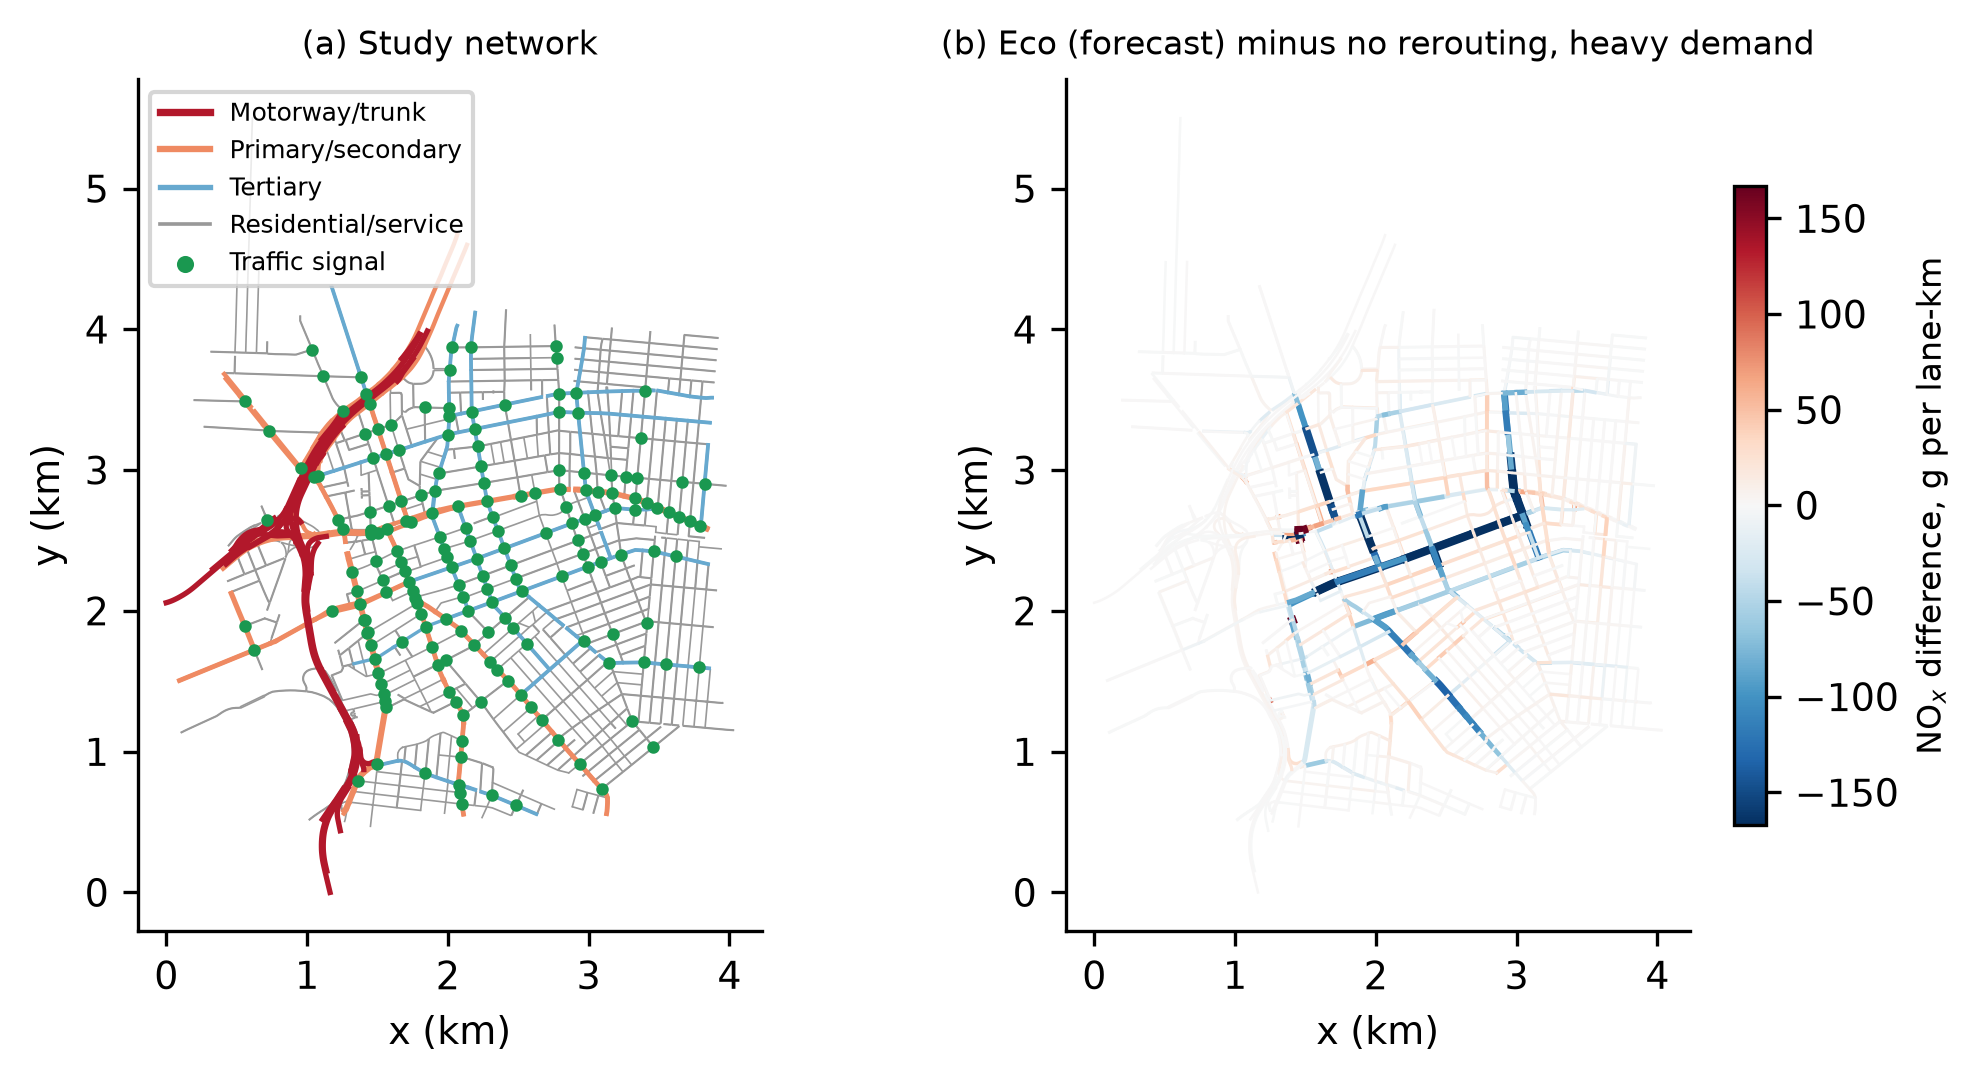
\includegraphics[width=0.88\textwidth]{paper_area_map_heavy.png}
\caption{(a) The Flushing study network by road class, with traffic signals. (b) Mean per-edge NO$_x$ difference over
valid seed pairs, forecast eco-routing minus no rerouting, heavy demand (red: more NO$_x$; blue: less).}
\label{fig:area}
\end{figure*}

\begin{table}[t]
\centering\footnotesize
\caption{The Two Network Codings (Modal Speed per Road Class, with Its Share of the Class's Lane-km)}
\label{tab:networks}
% Generated by `python -m nycemis report` from result files; do not edit by hand.
\begin{tabular}{lrr}
\toprule
 & As built & NYC-coded \\
\midrule
Edges / lane-km & 2,316 / 300 & 2,316 / 300 \\
Signal programs & 176 & 176 \\
Priority junctions & 686 & 130 \\
Stop-controlled junctions & 0 & 558 \\
Prim./sec. speed, km/h & 100 (70\%) & 40 (87\%) \\
Tertiary speed, km/h & 80 (96\%) & 40 (98\%) \\
Resid./service speed, km/h & 50 (96\%) & 40 (100\%) \\
\bottomrule
\end{tabular}

\end{table}

\subsection{Demand and fleet}
Trips are generated per vehicle class with the Web Wizard's options of SUMO's \texttt{randomTrips} tool and routed
explicitly; each vehicle's HBEFA~4.2 emission class is fixed in the route file, so every condition shares the fleet.
Departures fall within one hour. Three demand levels are calibrated on pilot seeds to target values of the relative
speed ratio (RSR), the ratio of ideal to actual travel time relative to a near-empty network (Table~\ref{tab:demand}).

\begin{table}[t]
\centering\footnotesize
\caption{Calibrated Demand Levels (Density in veh/h/km of Road; RSR Achieved on Pilot Seeds)}
\label{tab:demand}
% Generated by `python -m nycemis report` from result files; do not edit by hand.
\begin{tabular}{lrrrrr}
\toprule
 & & \multicolumn{2}{c}{As built} & \multicolumn{2}{c}{NYC-coded} \\
\cmidrule(lr){3-4}\cmidrule(lr){5-6}
Level & Target & Density & RSR & Density & RSR \\
\midrule
Light & 0.95 & 10 & 0.947 & 12 & 0.942 \\
Moderate & 0.85 & 16 & 0.849 & 16 & 0.845 \\
Heavy & 0.72 & 20.75 & 0.719 & 18 & 0.805$^{a}$ \\
\bottomrule
\end{tabular}
\\[2pt]
\parbox{\columnwidth}{\scriptsize $^{a}$Target not reached: denser demand made pilot runs fail the validity rule, so the
most congested valid density is used.}
\end{table}

\section{Methodology}\label{sec:methods}
\subsection{Matched protocol}
Every condition of a seed shares the network, a byte-identical route file, the fleet, the SUMO seed and the options,
and every run continues until all vehicles have arrived. A run is valid if at least \ValidCompletionPct\% of its
vehicles complete their trips and at most \ValidTeleportPct\% are teleported. The primary outcome is total NO$_x$ from
SUMO's per-trip emission output; travel time, its 95th percentile, departure delay, vehicle-kilometres and CO$_2$ are
secondary.

\subsection{Controllers}
Table~\ref{tab:controllers} lists the six conditions. The eco-routing controllers set a routing weight on every edge
every \ReroutePeriodS~s,
\begin{equation}
w_e = (1-\alpha)\,\tau_e + \alpha\,\bar\tau\,\frac{m_e}{\bar m},
\label{eq:weight}
\end{equation}
where $\tau_e$ is the edge's travel time from its time-mean speed over the last \TauAvgS~s (floored at free-flow time,
as SUMO's rerouting device averages), $m_e$ the NO$_x$ a vehicle emits traversing the edge, and bars denote network
means. Each vehicle is rerouted every \ReroutePeriodS~s with SUMO's travel-time router on these weights, so at
$\alpha = 0$ the controllers reduce to travel-time rerouting. $\alpha^*$ was chosen on validation seeds as the value
minimising NO$_x$ with mean travel time at most \AlphaTTBudgetPct\% above travel-time rerouting's.

\begin{table}[t]
\centering\footnotesize
\caption{Conditions (All Controllers Act on All Vehicles)}
\label{tab:controllers}
\begin{tabular}{@{}p{0.3\columnwidth}p{0.64\columnwidth}@{}}
\toprule
Condition & Rule \\
\midrule
No rerouting & Vehicles keep their free-flow routes. \\
Travel-time rerouting & SUMO's rerouting device, default adaptation. \\
Random placebo & Weight (\ref{eq:weight}) with the emission term replaced by noise ($\eta^* = \EtaStar$), matched in
route-change rate to forecast eco-routing on validation seeds. \\
Eco-routing (measured) & $m_e$ measured over the last minute and smoothed; $\alpha^* = \AlphaStarReactive$. \\
Eco-routing (forecast) & $m_e$ forecast for the next \HorizonS~s from traffic-state features; $\alpha^* =
\AlphaStarML$. \\
Legacy rule & A random forest predicts each vehicle's NO$_x$ from its other pollutants every step; above
\LegacyThreshold~mg/s the vehicle gets SUMO's default route search. \\
\bottomrule
\end{tabular}
\end{table}

\subsection{Forecaster}
Gradient-boosted trees forecast each edge's NO$_x$ per vehicle-second, mean speed and NO$_x$ density for the next
minute from sensor-like features only (vehicle counts, speeds, halting, waiting time, their lags, their upstream and
downstream neighbours, and static attributes), with no emission information. They are trained on runs under a mix of
controllers, so that training data contain controller-induced traffic states, and tuned on validation seeds.
Baselines are persistence, an exponential moving average, the per-edge historical mean of the training data and ridge
regression.

\subsection{Experimental design and preregistration}
Seeds are disjoint across pilot, training, validation and test roles (Table~\ref{tab:design}). The comparisons, the
$\alpha^*$ rule, the test seeds, the sample size and the analysis code (by hash) were frozen in a tagged commit before
any test seed ran. The tag is in the project's own repository, whose history was rewritten after the study
(commit hashes changed; dates and tags were kept), so the timing of the freeze rests on that record. The pilot's spread of paired changes (SD \PilotSD\%) gave $n = \ConfirmatoryN$ test seeds per
condition and level, the cap of the preregistered rule. Every departure from the plan is logged with its reason.

\begin{table}[t]
\centering\footnotesize
\caption{Experiments and Seed Sets}
\label{tab:design}
% Generated by `python -m nycemis report` from result files; do not edit by hand.
\begin{tabular}{llrr}
\toprule
Experiment & Seeds & Cond. & Runs \\
\midrule
Pilot & 9000--9004 & 7 & 105 \\
Training data & 0--23, 100--111 & 4 & 432 \\
Validation & 100--111 & 17 & 612 \\
Confirmatory & 200--259 & 6 & 1,080 \\
Legacy recount & 9000--9004 & 1 & 15 \\
Sensitivity & 200--259 & 3 & 540 \\
\bottomrule
\end{tabular}

\end{table}

\subsection{Statistical analysis}
For each seed we compute the percent change of total NO$_x$ against the reference condition. Four preregistered
comparisons are tested at each demand level: PC1 (legacy rule vs no rerouting) and PC4 (forecast vs measured
eco-routing) with two one-sided tests (TOST) for equivalence within $\pm$\SESOI\%, and PC2 (forecast eco-routing vs no
rerouting) and PC3 (vs travel-time rerouting) with two-sided Wilcoxon signed-rank tests. The \TestsInFamily\ tests
form one Holm family at \FamilywiseAlpha, with BCa intervals. The planned power at $n = \ConfirmatoryN$ was
\PowerAtNSup\% for a true change of \SESOI\%; the observed SDs of paired changes (\ObservedSDMin\% to
\ObservedSDMax\%) gave much higher precision. Everything beyond PC1--PC4 is exploratory.

\subsection{Legacy replication}
The legacy rule is reproduced as a condition (Table~\ref{tab:controllers}) with its random forest retrained on the
same kind of records. Its ``legacy metric'' sums every NO$_x$ record of a full no-rerouting run against the rerouting
run's first \LegacyControlledSteps~s, as the 2024 notebook did; the ``matched metric'' compares complete runs.

\subsection{Network-coding sensitivity experiment}\label{sec:sensdesign}
On a recoded copy of the network (Table~\ref{tab:networks}, ``NYC-coded''), the \SensEdgesSpeedChanged\ edges that
carried a road-type default speed get New York City's default limit of 25~mph, which applies to streets without a
posted limit \cite{nycdot2014speed}; the \SensEdgesTagged\ edges with an OSM speed tag keep it; and the
\SensJunctionsStop\ unsignalised junctions entered by a residential, unclassified or service street get a stop on
their minor approaches (a modelling assumption). Edges, lanes and signals are unchanged, and demand was recalibrated
to the same targets (Table~\ref{tab:demand}). No rerouting, travel-time rerouting and measured eco-routing ($\alpha^* =
\AlphaStarReactive$) ran on the same \ConfirmatoryN\ test seed numbers; forecast eco-routing did not, because its
forecaster takes the speed limits as inputs. The pre-specified reading: the reduction ``persists'' at a level if the
95\% interval of measured eco-routing vs travel-time rerouting lies below zero.

\section{Results}\label{sec:results}
\subsection{RQ1: the legacy result is a measurement artifact}
In the 2024 notebook the rerouting runs covered \LegacyRowRatioRF\% as many vehicle-steps as the baseline, and
\LegacyRepeatUnchanged\ of \LegacyRepeatCalls\ repeated reroute calls returned the unchanged route. Its predictor is
near-deterministic ($R^2 = \LegacyRFRTwo$ on a random split, \LegacyRFRunSplitRTwo\ split by run), because NO$_x$ is
predicted from other outputs of the same emission model at the same instant. Replicated under the matched protocol,
the legacy metric still reports a large drop while the matched metric shows none (Table~\ref{tab:legacy}), and the
rule is close to a no-op: \LegacyRecountChanges\ of \LegacyRecountCalls\ reroute calls changed a path
(\LegacyRecountRate\%). PC1 confirms equivalence to no rerouting at every level (Table~\ref{tab:pc}).

\begin{table}[t]
\centering\footnotesize
\caption{Legacy Replication on the Test Seeds (Matched Change: Negative Means Lower NO$_x$; $n$ = Seeds)}
\label{tab:legacy}
% Generated by `python -m nycemis report` from result files; do not edit by hand.
\begin{tabular}{lrrlrl}
\toprule
 & & \multicolumn{2}{c}{Legacy metric: drop, \%} & \multicolumn{2}{c}{Matched: change, \%} \\
\cmidrule(lr){3-4}\cmidrule(lr){5-6}
Level & $n$ & Mean & Range & Mean & Range \\
\midrule
Light & 60 & 76.6 & 73.8--81.2 & +0.07 & $-$1.3 to +1.2 \\
Moderate & 60 & 77.8 & 75.8--79.4 & $-$0.15 & $-$2.6 to +4.0 \\
Heavy & 60 & 79.1 & 76.6--82.4 & +0.32 & $-$12.3 to +8.7 \\
\bottomrule
\end{tabular}

\end{table}

\subsection{RQ3: preregistered comparisons}
Table~\ref{tab:pc} and Fig.~\ref{fig:forest} give the twelve preregistered tests. Forecast eco-routing lowered total
NO$_x$ against no rerouting and against travel-time rerouting at every level. Equivalence with measured eco-routing
(PC4) was not shown; its 90\% intervals lie below $-$\SESOI\% at light and moderate demand, so the forecast version
emitted less by more than the margin there (exploratory reading).

\begin{table*}[t]
\centering\footnotesize
\caption{Preregistered Comparisons: Mean Paired Change in Total NO$_x$ with BCa Intervals and Holm-Adjusted $p$
(PC1, PC4: TOST Equivalence within $\pm$\SESOI\%; PC2, PC3: Wilcoxon)}
\label{tab:pc}
% Generated by `python -m nycemis report` from result files; do not edit by hand.
\begin{tabular}{lllrrllll}
\toprule
 & Comparison & Level & $n$ & Mean, \% & 95\% CI & 90\% CI & $p_\mathrm{Holm}$ & Outcome \\
\midrule
PC1 & Legacy rule vs no rerouting & Light & 60 & +0.07 & [$-$0.06, +0.21] & [$-$0.04, +0.19] & $<10^{-9}$ & equivalent within $\pm$2\% \\
 &  & Moderate & 60 & $-$0.15 & [$-$0.40, +0.15] & [$-$0.36, +0.10] & $<10^{-9}$ & equivalent within $\pm$2\% \\
 &  & Heavy & 58 & +0.65 & [$-$0.24, +1.40] & [$-$0.09, +1.28] & 0.002 & equivalent within $\pm$2\% \\
\addlinespace
PC2 & Eco (forecast) vs no rerouting & Light & 60 & $-$9.75 & [$-$9.95, $-$9.54] & -- & $<10^{-9}$ & reduction \\
 &  & Moderate & 60 & $-$11.00 & [$-$11.32, $-$10.70] & -- & $<10^{-9}$ & reduction \\
 &  & Heavy & 58 & $-$14.95 & [$-$15.67, $-$14.35] & -- & $<10^{-9}$ & reduction \\
\addlinespace
PC3 & Eco (forecast) vs travel time & Light & 60 & $-$9.25 & [$-$9.43, $-$9.06] & -- & $<10^{-9}$ & reduction \\
 &  & Moderate & 60 & $-$8.49 & [$-$8.65, $-$8.33] & -- & $<10^{-9}$ & reduction \\
 &  & Heavy & 60 & $-$8.07 & [$-$8.27, $-$7.85] & -- & $<10^{-9}$ & reduction \\
\addlinespace
PC4 & Eco (forecast) vs eco (measured) & Light & 60 & $-$2.76 & [$-$3.03, $-$2.48] & [$-$2.99, $-$2.53] & 1.000 & equivalence not shown \\
 &  & Moderate & 60 & $-$2.30 & [$-$2.56, $-$2.03] & [$-$2.52, $-$2.07] & 1.000 & equivalence not shown \\
 &  & Heavy & 60 & $-$2.15 & [$-$2.40, $-$1.90] & [$-$2.36, $-$1.93] & 1.000 & equivalence not shown \\
\bottomrule
\end{tabular}

\end{table*}

\begin{figure}[t]
\centering
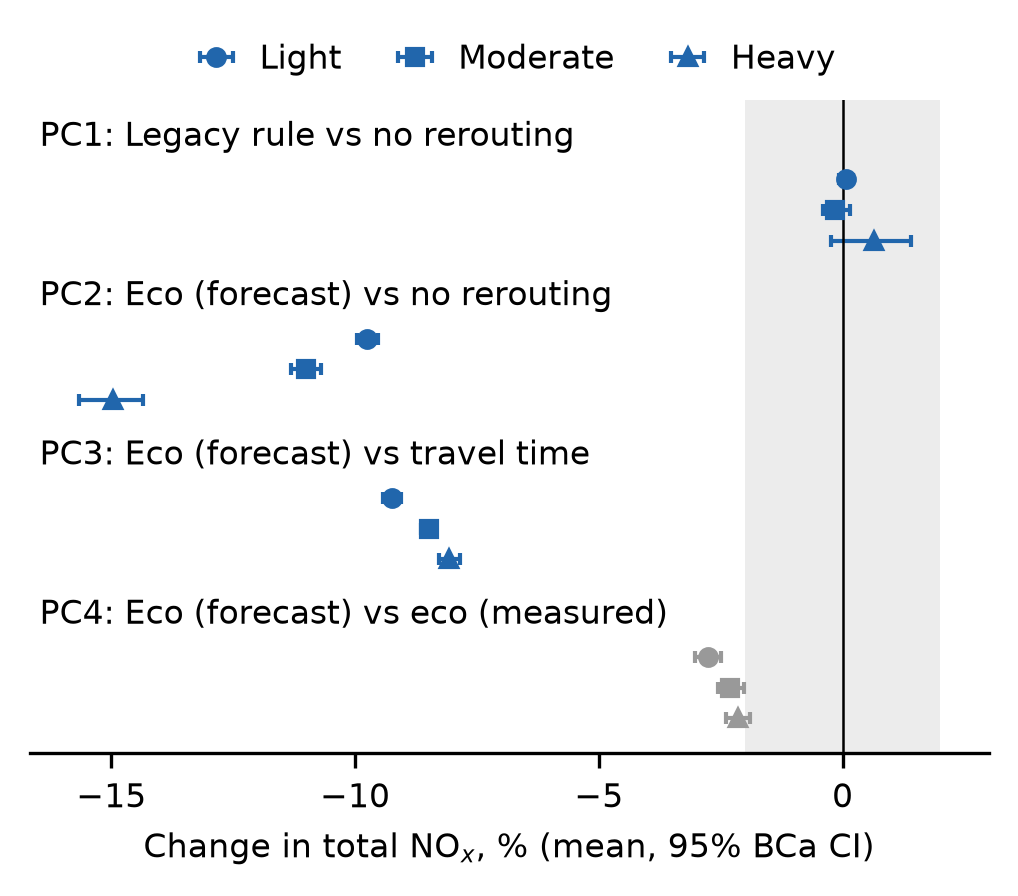
\includegraphics[width=\columnwidth]{paper_forest_pc_compact.png}
\caption{Preregistered comparisons, mean and 95\% BCa interval (blue: Holm test rejects; grey: equivalence not shown;
shaded band: equivalence margin).}
\label{fig:forest}
\end{figure}

\textit{Cost and controls.} Against travel-time rerouting, forecast eco-routing cost a few percent of mean travel
time and more at the 95th percentile, and roughly doubled the small mean departure delay (Table~\ref{tab:cost}). It
used fewer vehicle-kilometres and lowered CO$_2$, and it lowered NO$_x$ against the random placebo by about a tenth, so
rerouting as such does not explain the reduction.

\begin{table*}[t]
\centering\footnotesize
\caption{Cost and Controls (Exploratory): Mean Paired Change with 95\% BCa Interval, and Mean Departure Delay}
\label{tab:cost}
% Generated by `python -m nycemis report` from result files; do not edit by hand.
\begin{tabular}{llll}
\toprule
Quantity (eco-routing with forecast unless stated) & Light & Moderate & Heavy \\
\midrule
Mean travel time vs travel time, \% & +1.8 [+1.5, +2.1] & +2.0 [+1.8, +2.3] & +1.1 [+0.8, +1.5] \\
95th-percentile travel time vs travel time, \% & +3.7 [+2.9, +4.4] & +7.2 [+6.5, +8.0] & +6.5 [+5.7, +7.6] \\
Mean travel time vs no rerouting, \% & +2.8 [+2.5, +3.1] & $-$0.7 [$-$1.4, $-$0.1] & $-$10.9 [$-$12.4, $-$9.7] \\
Vehicle-km vs no rerouting, \% & $-$2.4 [$-$2.4, $-$2.3] & $-$2.3 [$-$2.3, $-$2.3] & $-$2.2 [$-$2.3, $-$2.2] \\
CO$_2$ vs no rerouting, \% & $-$7.8 [$-$8.0, $-$7.7] & $-$9.2 [$-$9.4, $-$9.0] & $-$12.9 [$-$13.5, $-$12.4] \\
NO$_x$ vs random placebo, \% & $-$10.4 [$-$10.6, $-$10.2] & $-$10.1 [$-$10.3, $-$9.9] & $-$10.0 [$-$10.2, $-$9.8] \\
Eco (measured): NO$_x$ vs no rerouting, \% & $-$7.2 [$-$7.4, $-$6.9] & $-$8.9 [$-$9.3, $-$8.6] & $-$13.1 [$-$13.7, $-$12.5] \\
Travel time: NO$_x$ vs no rerouting, \% & $-$0.6 [$-$0.7, $-$0.4] & $-$2.7 [$-$3.1, $-$2.4] & $-$7.5 [$-$8.2, $-$6.9] \\
Departure delay, eco (forecast) / travel time, s & 1.3 / 1.0 & 2.7 / 1.4 & 4.0 / 2.1 \\
\bottomrule
\end{tabular}

\end{table*}

\subsection{RQ5: the reduction is a shift onto residential streets}
Per-edge NO$_x$ shows where the reduction comes from (Table~\ref{tab:spatial}, Fig.~\ref{fig:roadclass}, top row).
Forecast eco-routing roughly doubled NO$_x$ and vehicle-hours on residential and service streets and cut NO$_x$ on
tertiary and arterial roads. Holding each road class's NO$_x$ per vehicle-hour at the paired no-rerouting run's value,
the change in where vehicles spend their time accounts for \CompositionLight\%, \CompositionModerate\% and
\CompositionHeavy\% of the edge-NO$_x$ change (above 100 means NO$_x$ per vehicle-hour within classes rose). Measured
eco-routing shifts NO$_x$ the same way. Fig.~\ref{fig:area}(b) shows the pattern: reductions on the arterial corridors,
smaller increases spread over side streets.

\begin{table}[t]
\centering\footnotesize
\caption{Where the Change Occurs: Forecast Eco-Routing vs No Rerouting, Per-Edge NO$_x$ (Mean Paired Change)}
\label{tab:spatial}
% Generated by `python -m nycemis report` from result files; do not edit by hand.
\begin{tabular}{lrrr}
\toprule
vs no rerouting & Light & Mod. & Heavy \\
\midrule
Resid./service NO$_x$, \% & +90 & +95 & +94 \\
Resid./service veh-h, \% & +92 & +96 & +92 \\
Resid. share of NO$_x$, \% & 15$\to$31 & 14$\to$32 & 14$\to$33 \\
Tertiary NO$_x$, \% & $-$41 & $-$44 & $-$50 \\
Primary/secondary NO$_x$, \% & $-$20 & $-$20 & $-$23 \\
Edge NO$_x$, \% & $-$10.8 & $-$12.0 & $-$16.8 \\
Explained by class mix, \% & 54 & 72 & 108 \\
\bottomrule
\end{tabular}

\end{table}

\begin{figure*}[t]
\centering
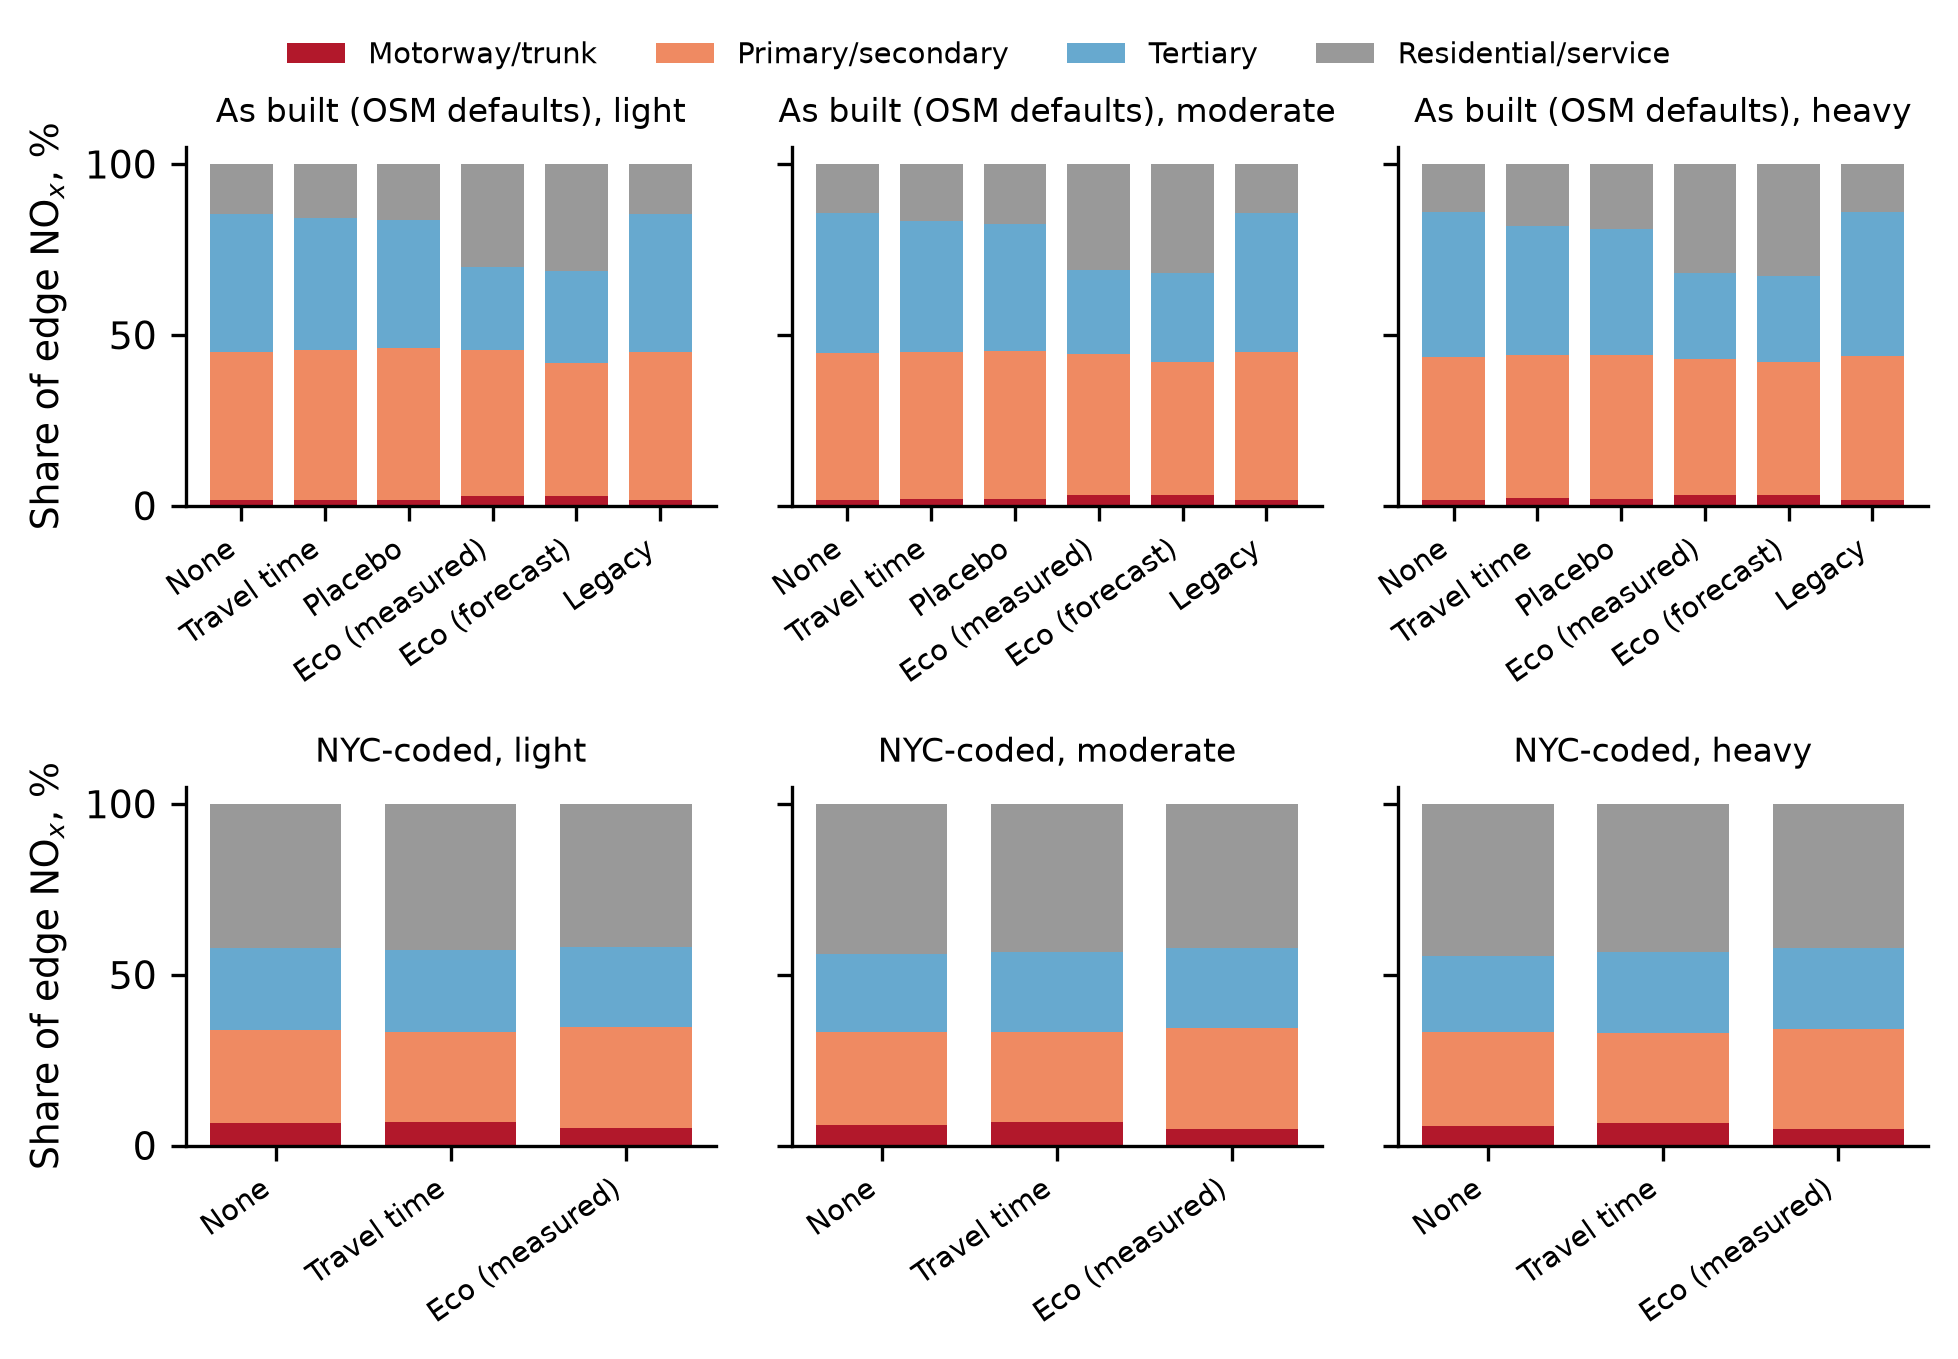
\includegraphics[width=0.74\textwidth]{paper_road_class.png}
\caption{Share of edge NO$_x$ by road class, mean over test seeds: network as built (top) and NYC-coded network
(bottom, sensitivity experiment).}
\label{fig:roadclass}
\end{figure*}

\subsection{RQ2: the forecast adds little over a per-edge average}
On \TestRuns\ test-seed runs the forecaster clearly beats persistence, but for NO$_x$ per vehicle-second, the quantity
the controller's emission cost uses, it \ForecastVerdictR\ the per-edge historical mean (Table~\ref{tab:forecast}).
It beats the historical mean for speed and NO$_x$ density, and it ranks hotspots (edge-windows whose next-window NO$_x$
density exceeds the 95th percentile of the training edge-windows) better than every baseline, with the highest PR-AUC.

\begin{table}[t]
\centering\footnotesize
\caption{Forecast Accuracy on the Test Seeds: Mean Absolute Error, Hotspot PR-AUC, and Skill (1 $-$ MAE Ratio,
95\% Cluster-Bootstrap Interval over Runs)}
\label{tab:forecast}
% Generated by `python -m nycemis report` from result files; do not edit by hand.
\begin{tabular}{@{}lrrrr@{}}
\toprule
 & \multicolumn{3}{c}{MAE, test seeds} & Hotspot \\
\cmidrule(lr){2-4}\cmidrule(l){5-5}
Model & NO$_x$/veh-s & Speed & NO$_x$ dens. & PR-AUC \\
\midrule
Boosted trees (ours) & 3.825 & 2.347 & 0.463 & 0.255 \\
Per-edge hist. mean & 3.816 & 2.426 & 0.592 & 0.148 \\
Persistence & 4.611 & 3.643 & 0.639 & 0.128 \\
Moving average & 4.473 & 3.223 & 0.605 & 0.152 \\
Ridge & 3.954 & 2.864 & 0.496 & 0.182 \\
\addlinespace
\multicolumn{5}{@{}l}{\emph{Skill vs per-edge historical mean, 95\% interval}} \\
\quad Lower bound & $-$0.003 & +0.031 & +0.210 &  \\
\quad Upper bound & $-$0.002 & +0.035 & +0.225 &  \\
\bottomrule
\end{tabular}

\end{table}

\subsection{Network-coding sensitivity: the effect reverses}
On the NYC-coded network, measured eco-routing no longer lowers NO$_x$ against travel-time rerouting: at every level its
95\% interval lies above zero (Table~\ref{tab:sens}, Fig.~\ref{fig:sens}). Against no rerouting its reduction shrinks or
vanishes, while travel-time rerouting lowers NO$_x$ more than on the original network. With the default limit on every
urban street, free-flow routes already use residential streets heavily (Fig.~\ref{fig:roadclass}, bottom), and
eco-routing no longer shifts NO$_x$ onto them; its travel-time cost grew. Of the 540 runs, \SensInvalidRuns\ failed
the validity rule (pairs excluded). By the pre-specified reading, the reduction does not persist at any level; light
and moderate demand, where both networks are equally congested, show it as clearly as heavy demand.

\begin{table*}[t]
\centering\footnotesize
\caption{Sensitivity Experiment: Change in Total NO$_x$ on the Network as Built (Confirmatory Runs) and on the
NYC-Coded Network, and Their Difference (NYC-Coded Minus As Built; Independent Samples, Percentile Bootstrap)}
\label{tab:sens}
% Generated by `python -m nycemis report` from result files; do not edit by hand.
\begin{tabular}{lllllr}
\toprule
Total NO$_x$ change, \% & Level & As built & NYC-coded (95\% CI) & Difference (95\% CI) & $n$ \\
\midrule
Eco (measured) vs travel time & Light & $-$6.7 & +2.9 [+2.7, +3.1] & +9.5 [+9.2, +9.8] & 60 \\
 & Moderate & $-$6.3 & +3.4 [+3.2, +3.6] & +9.7 [+9.5, +10.0] & 60 \\
 & Heavy & $-$6.1 & +3.6 [+3.3, +3.7] & +9.6 [+9.3, +9.9] & 59 \\
\addlinespace
Eco (measured) vs no rerouting & Light & $-$7.2 & +1.1 [+0.6, +1.5] & +8.2 [+7.7, +8.7] & 60 \\
 & Moderate & $-$8.9 & $-$3.0 [$-$3.7, $-$2.3] & +5.9 [+5.1, +6.7] & 59 \\
 & Heavy & $-$13.1 & $-$5.2 [$-$5.8, $-$4.6] & +7.8 [+7.0, +8.7] & 56 \\
\addlinespace
Travel time vs no rerouting & Light & $-$0.6 & $-$1.7 [$-$2.2, $-$1.4] & $-$1.2 [$-$1.6, $-$0.8] & 60 \\
 & Moderate & $-$2.7 & $-$6.2 [$-$6.9, $-$5.5] & $-$3.4 [$-$4.2, $-$2.7] & 59 \\
 & Heavy & $-$7.5 & $-$8.5 [$-$9.1, $-$7.9] & $-$1.0 [$-$1.9, $-$0.1] & 57 \\
\addlinespace
Residential NO$_x$, eco (measured) vs none & Light & +89 & +0 [$-$1, +2] &  &  \\
 & Moderate & +95 & $-$7 [$-$9, $-$6] &  &  \\
 & Heavy & +93 & $-$11 [$-$12, $-$10] &  &  \\
\bottomrule
\end{tabular}

\end{table*}

\begin{figure}[t]
\centering
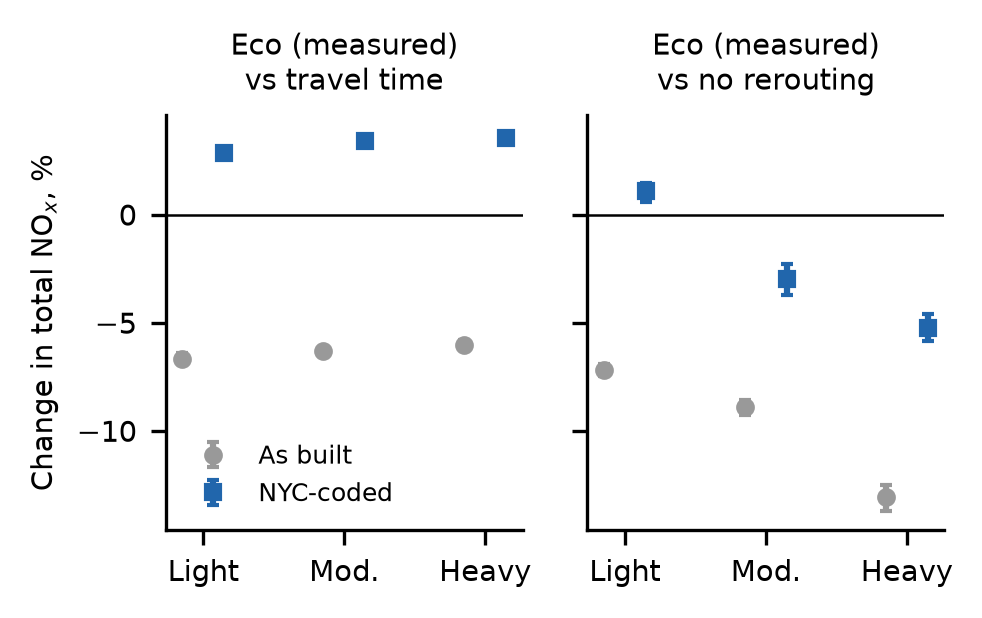
\includegraphics[width=\columnwidth]{paper_sensitivity_compact.png}
\caption{Measured eco-routing on the network as built and on the NYC-coded network: change in total NO$_x$ (mean, 95\% BCa interval). Travel-time rerouting vs no rerouting is in Table~\ref{tab:sens}.}
\label{fig:sens}
\end{figure}

\section{Discussion}\label{sec:discussion}
\textit{Principal findings.} The 2024 reduction was produced by its measurement: a full baseline was compared with
truncated runs, and the intervention did not change routes. Under a matched, preregistered protocol, forecast
eco-routing reduced simulated network NO$_x$ on the network as built, at a modest travel-time cost, and beat a
placebo matched in route-change rate. But the reduction is mostly a relocation of traffic onto residential streets,
and on a network coded like New York City's streets the same kind of controller increases NO$_x$ relative to plain
travel-time rerouting.

\textit{Why network coding matters.} An eco-router minimises the emission cost of a route. In the OSM-derived
network, arterials carry SUMO's type-default speeds of \SpeedTertiary--\SpeedPrimSec~km/h and stop at signals, so
their per-vehicle emission cost is high, while residential streets coded at \SpeedResid~km/h without stop control are
cheap; the router exploits exactly that contrast. With 25~mph on arterials and residential streets alike, and stops
on minor approaches, the contrast largely disappears: residential streets are already used by free-flow routes, and
detours add stop-and-go and distance without a lower emission rate. The controller's effect is therefore inseparable
from how the network encodes speed and junction control, attributes that OpenStreetMap often lacks and conversion
tools fill with defaults.

\textit{Implications.} Simulation studies of eco-routing should (i) compare runs of equal scope, (ii) verify that the
intervention changes behaviour, (iii) include travel-time and placebo baselines, (iv) report where emissions move,
not only totals, and (v) test the result against the network attributes it depends on. A routing objective that
counts only total network NO$_x$ rewards displacement onto residential streets; deployment-oriented studies need an
exposure-aware objective and dispersion modelling, which this study does not have.

\textit{The forecast.} The controller's emission cost uses forecast NO$_x$ per vehicle-second, for which the
forecaster does not beat a per-edge historical average. Forecast eco-routing emitted less than measured eco-routing at
some levels, but no preregistered condition isolates the forecast, and a learned per-edge prior is a plausible source
of that difference; we do not attribute it to forecasting.

\section{Threats to Validity}\label{sec:threats}
\textit{Construct:} the outcome is simulated tailpipe emission mass from European (HBEFA) models, not concentration,
exposure or health; road-class results cover edges, not junction lanes. \textit{Internal:} conditions are paired by
seed and share route files, the analysis code was frozen before the test seeds, and post-hoc additions are labelled
exploratory and logged, among them a corrected route-change counter for the legacy replication. \textit{External:}
demand is synthetic, uncalibrated to traffic counts and lasts one hour; drivers comply fully; only one district was
studied; the network comes from OpenStreetMap and its coding changes the result; the recoded network's stop control
is an assumption, forecast eco-routing was not tested on it, and neither coding was validated against measured
speeds. \textit{Statistical:} intervals are narrow because runs are paired and seeds many; the sensitivity experiment
is exploratory and uncorrected for multiplicity, and its heavy-demand comparison mixes coding and congestion.

\section{Conclusion and Future Work}\label{sec:conclusion}
An audit and a matched replication showed that reported simulated NO$_x$ reductions of \LegacyNOxDropRF\% and
\LegacyNOxDropXGB\% from ML-triggered rerouting were a measurement artifact. A preregistered rebuild found that
emission-aware rerouting does lower simulated NO$_x$ on the network as built, but mostly by moving traffic onto
residential streets, with a forecaster that adds little over a per-edge average; a sensitivity experiment showed that
the effect reverses when the network is coded like New York City's streets. The robust contribution is
methodological: simulated eco-routing benefits should be reported together with matched protocols, placebo controls,
the spatial redistribution of emissions and their sensitivity to network coding. Future work should calibrate network
speeds and junction controls against measured data, add exposure-aware routing objectives, isolate the value of the
forecast with a shuffled-forecast control, and test transfer to other districts and partial compliance.

\balance
\section*{Data and Code Availability}
Code, configurations, frozen inputs with SHA-256 hashes, the preregistration (git tag \texttt{prereg-v1}), the
sensitivity plan (tag \texttt{sensitivity-v1}), the deviation log and every result file are in the project
repository; each stage is one command, and every number in this paper is generated from result files.

\section*{Acknowledgment}
The 2024 project audited here was the authors' NYIT DTSC 870 course project, supervised by Prof.~X.~Huang (NYIT).
Map data \copyright\ OpenStreetMap contributors, ODbL.

\paragraph{Use of AI tools.} The study's software (simulation harness, controllers, forecaster pipeline, statistical
analysis, tests, and the scripts that generate this paper's tables, figures and numbers) was written with Claude
(Anthropic), an AI coding assistant used through Claude Code, under the authors' direction, and the text of this
paper was drafted with the same assistant. The authors set the research questions, approved the preregistered
protocol and the automated checks every result must pass, approved the final text, and take full responsibility
for the content. The assistant made a study of this scale practical for two authors; every reported number is
generated from the result files rather than typed.

\bibliographystyle{IEEEtran}
\bibliography{../refs}
\end{document}
